\documentclass{article}


% if you need to pass options to natbib, use, e.g.:
%     \PassOptionsToPackage{numbers, compress}{natbib}
% before loading neurips_2023


% ready for submission
% \usepackage{neurips_2023}


% to compile a preprint version, e.g., for submission to arXiv, add add the
% [preprint] option:
    \usepackage[preprint]{neurips_2023}


% to compile a camera-ready version, add the [final] option, e.g.:
    % \usepackage[final]{neurips_2023}


% to avoid loading the natbib package, add option nonatbib:
  %  \usepackage[nonatbib]{neurips_2023}


\usepackage[utf8]{inputenc} % allow utf-8 input
\usepackage[T1]{fontenc}    % use 8-bit T1 fonts
\usepackage{hyperref}       % hyperlinks
\usepackage{url}            % simple URL typesetting
\usepackage{booktabs}       % professional-quality tables
\usepackage{amsfonts}       % blackboard math symbols
\usepackage{nicefrac}       % compact symbols for 1/2, etc.
\usepackage{microtype}      % microtypography
\usepackage{xcolor}         % colors
\usepackage{graphicx}       % Required for including graphics
\usepackage{subcaption}     % Required for subfigure environment
\usepackage{listings}       % Required for lstlisting environment


\title{BME1312 Project1 Report}


% The \author macro works with any number of authors. There are two commands
% used to separate the names and addresses of multiple authors: \And and \AND.
%
% Using \And between authors leaves it to LaTeX to determine where to break the
% lines. Using \AND forces a line break at that point. So, if LaTeX puts 3 of 4
% authors names on the first line, and the last on the second line, try using
% \AND instead of \And before the third author name.


\author{%
  Wenye Xiong \\
  2023533 \\
  \texttt{xiongwy2023@shanghaitech.edu.cn}
  \And
  Renyi Yang \\
  2023533030 \\
  \texttt{yangry2023@shanghaitech.edu.cn}
  \AND
  Jiaxing Wu \\
  2023533 \\
  \texttt{wujx2023@shanghaitech.edu.cn}
  \And
  Boyang Xia \\
  2023533073 \\
  \texttt{xiaby2023@shanghaitech.edu.cn}
  \AND
  Fengmin Yang \\
  2023533183 \\
  \texttt{yangfm2023@shanghaitech.edu.cn}
}

\begin{document}


\maketitle


\begin{abstract}
  This project uses deep learning to reconstruct high-quality dynamic MRI images
  from undersampled data. We propose a deep-learning-based denoising framework combining
  two independent UNet modules and a 3D ResNet to explore the temporal correlation.
  We generate variable density undersampling patterns with acceleration factor 5 and
  central k-space sampling, analyze the resulting aliasing artifacts, and evaluate
  reconstruction performance with PSNR and SSIM metrics. Additionally,
  we investigate the effects of dropout, dynamic learning rate schedules,
  and compare L1 versus L2 losses. Finally, we % TODO: for part(e)
\end{abstract}

\section{Variable Density Random Undersampling Pattern Generation and Aliasing Artifacts Analysis}
\textit{Note: }You may need \texttt{train.py}, line 29, function \texttt{variable\_density\_mask()}
and line 456, function \texttt{process\_data()} for reference in this section.

\subsection{Undersampling Pattern Generation}
We were asked to generate a variable density random undersampling mask $U$ matching the cine
dataset size, with acceleration factor 5 and 11 fully sampled central k-space lines per frame.
The mask values are 1 at sampled locations and 0 otherwise.

The provided code generate a 4D undersampling mask (shape [batch, frames, height, width]) using the following steps:
\begin{enumerate}
  \item Initialization: A zero-initialized mask is created with the input shape.
  \item Central Region Sampling: For each frame, 11 central k-space lines are
        sampled to retain low-frequency spatial information.
  \item Variable Density Probability Distribution: A quadratic probability density
        function is defined, decreasing with distance from the k-space center.
  \item Random Peripheral Sampling: The remaining lines are sampled randomly
        based on the probability distribution we obtained.
  \item Dynamic Frame Variability: Each dynamic frame independently generates
        unique random peripheral lines to ensure temporal incoherence of aliasing artifacts.
\end{enumerate}

\subsection{Undersampling Masks Plotting}
Figure 1 below shows the undersampling mask for one dynamic frame and undersampling masks in the ky-t dimension.

\begin{figure}[ht]
  \centering
  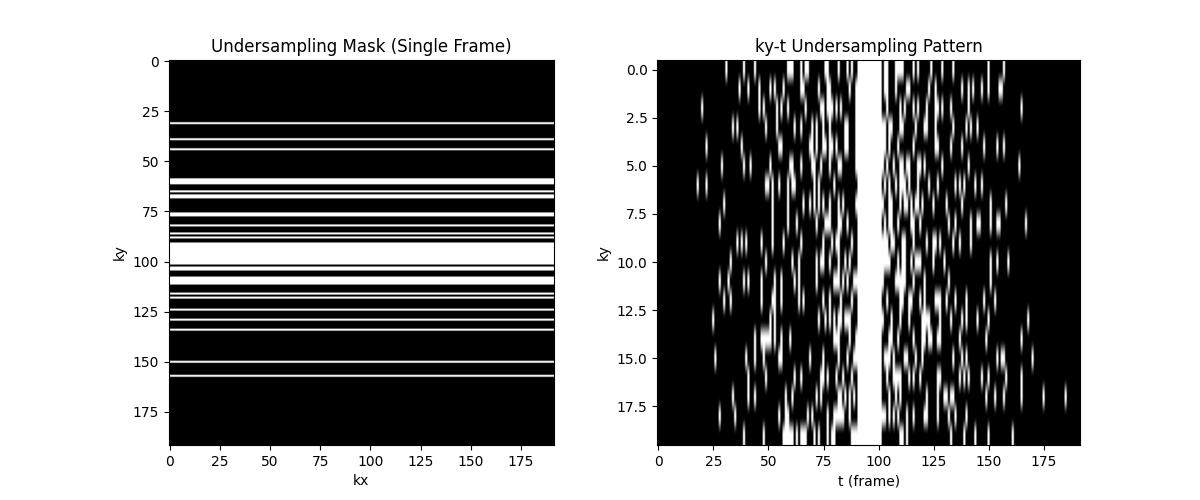
\includegraphics[width=\linewidth]{../assets/undersampling_mask.png}
  \caption{Undersampling Mask}
  \label{fig:undersampling mask for one dynamic frame and undersampling masks in the ky-t dimension}
\end{figure}

Thus we can see that the sampling mask is not the same for different dynamic frames.
That's because sampling positions are randomized per frame to disrupt coherent aliasing artifacts in time.

\subsection{Aliased Images Depiction and Comparison}
From the stem of this question we can know that, given a fully sampled image $m$,
the aliased image $b$ is computed as $F^{-1} U F m$, where $F$ is the Fourier transform.

In function \texttt{process\_data()}, we first load the dynamic MRI dataset dataset from the \texttt{cine.npz} file,
and convert the data into PyTorch tensor labels, which are used as ground truth for subsequent processing. Then we
call the function \texttt{variable\_density\_mask()} that we've just implemented to generate a mask,
and then apply the mask to the k-space data, and convert the fully sampled image data to the frequency
domain by Fourier transform (\texttt{image2kspace}). After that, we undersample the k-space data through the mask,
and perform an inverse Fourier transform (\texttt{kspace2image}) on the undersampled k-space to generate an aliased image.

Figure 2 below compares the fully sampled image, aliased image, and sampling mask in Fourier domain.
Here we choose the first 3 images generated to better compare the aliased images with the fully sampled image.

\begin{figure}[ht]
  \centering
  \begin{subfigure}[b]{\linewidth}
    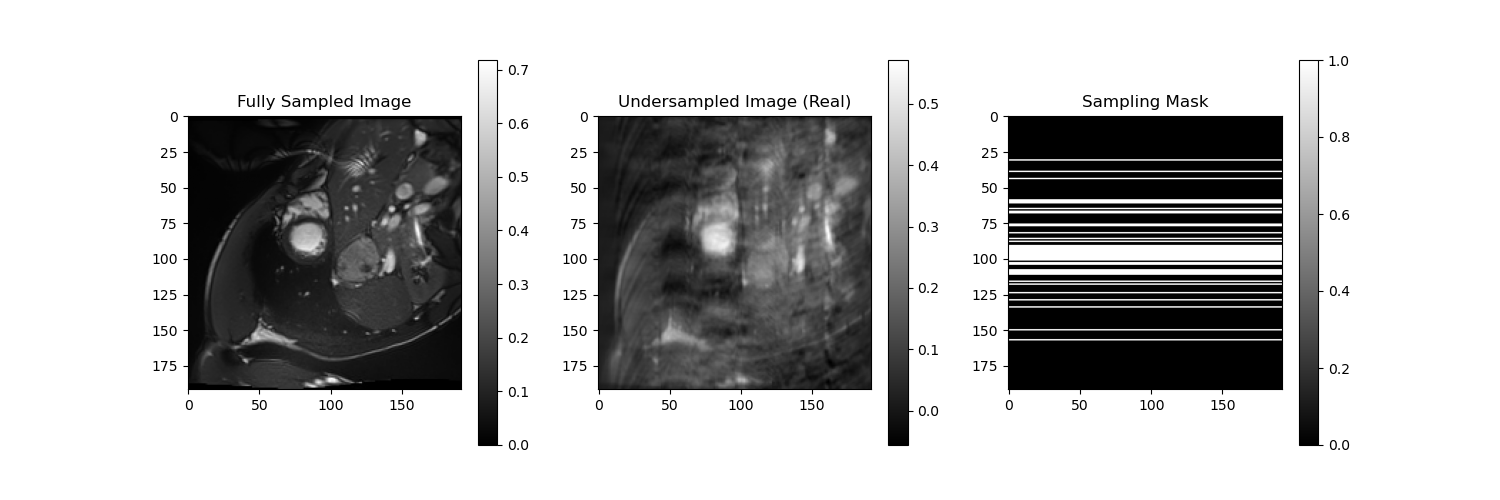
\includegraphics[width=\linewidth]{../assets/comparison_image_0.png}
    \caption{comparison image 0}
    \label{fig:comparison_image_0}
  \end{subfigure}
  \quad
  \begin{subfigure}[b]{\linewidth}
    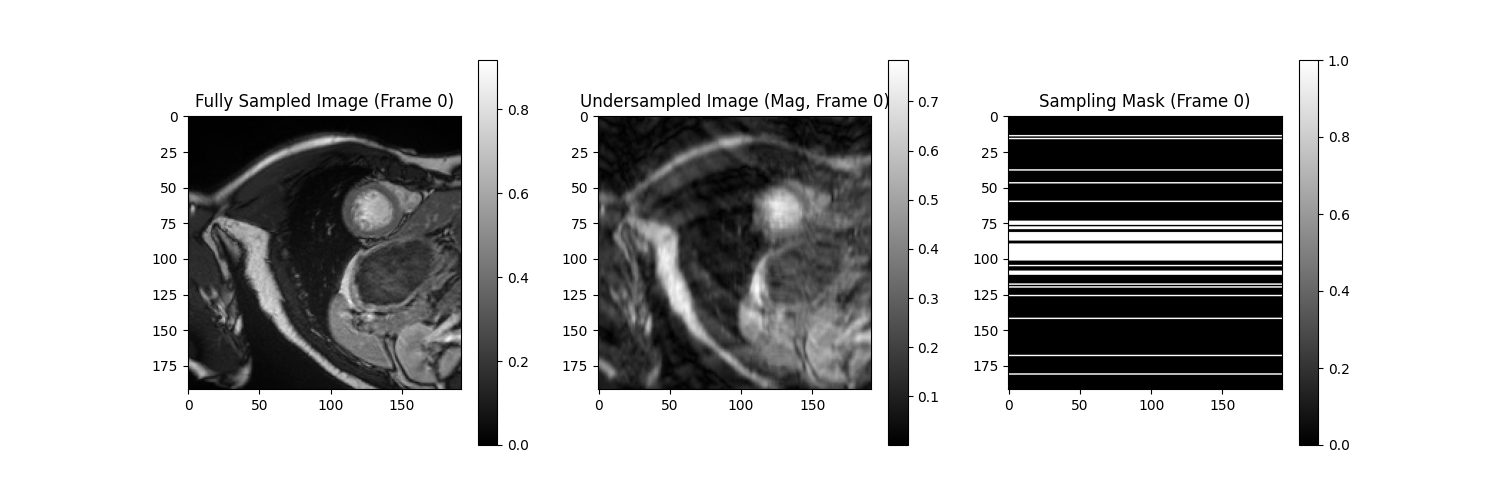
\includegraphics[width=\linewidth]{../assets/comparison_image_1.png}
    \caption{comparison image 1}
    \label{fig:comparison_image_1}
  \end{subfigure}
  \quad
  \begin{subfigure}[b]{\linewidth}
    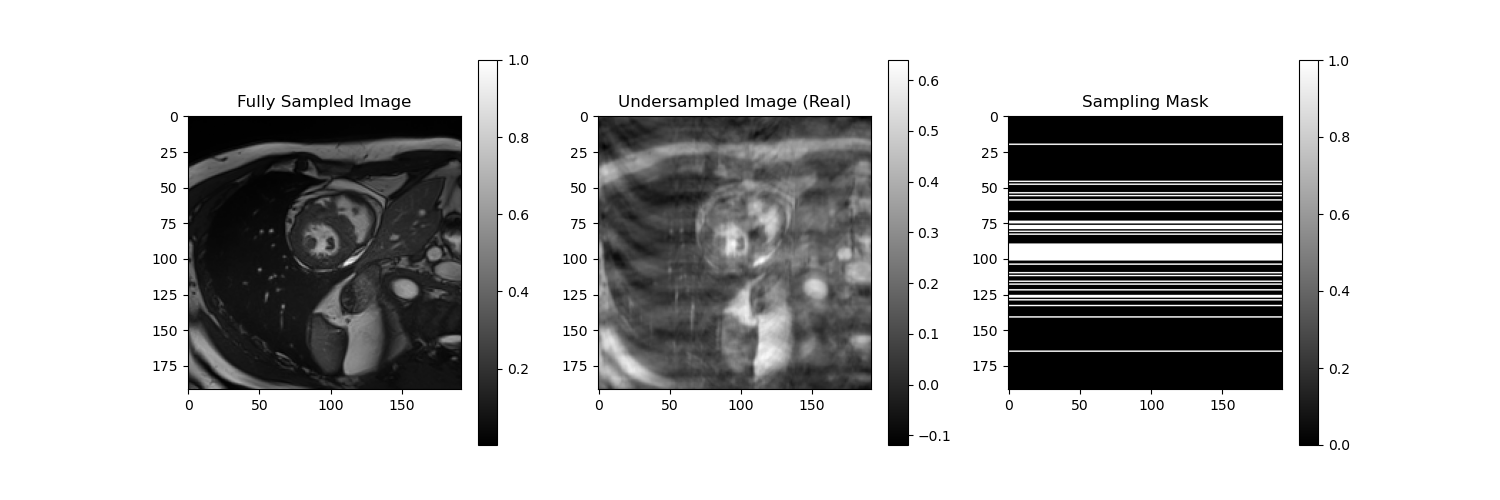
\includegraphics[width=\linewidth]{../assets/comparison_image_2.png}
    \caption{comparison image 2}
    \label{fig:comparison_image_2}
  \end{subfigure}
  \caption{compare the fully sampled images with aliased images}
\end{figure}

Description of aliased images: Since the low-frequency information in the center k-space
is usually better preserved, the main structure of the image is displayed more clearly;
however, due to the lack of high-frequency information, the edges of the image are
blurred with repetitive ripples (i.e., artifacts), especially in dynamic imaging,
where the artifacts vary with time frames.

Comparison of aliasing image and fully sampled image: fully sampled image retains
complete high-frequency information, with clear and detailed edges and no artifacts,
whereas aliasing image has reduced resolution due to insufficient high-frequency
sampling and produces artifacts.



\section{Dataset Partition, Denoising Network Construction and Evaluation}
\textit{Note: }You may need \texttt{train.py}, line 113, class \texttt{UNet};
line 345, class \texttt{ResNet} and line 497, function \texttt{train()}
for reference in this section. (Some related functions are also needed)

\subsection{Dataset Partition}

We know that the full dataset containing 200 samples is split into training, validation,
and testing sets with ratios 4:1:2, resulting in 114 training, 29 validation,
and 57 testing samples.

\subsection{CNN Network Designing and Training}
Our denoising network consists of two independent 2D UNet modules processing
separate input channels, whose outputs are stacked and fed into a 3D ResNet.
This design can effectively utilize both spatial information (2D UNet processing)
and temporal information (capturing dynamic changes via 3D ResNet) of the image
to better achieve the denoising task.

We train our network with Adam optimizer, initial learning rate $10^{-4}$,
weight decay $10^{-4}$, batch size 10, and $L2$ loss (MSE).
Note that training and validation losses are logged per epoch.

All the training loss and validation loss are recorded in the file named \texttt{output.txt}.
And the loss curves for 800 epochs are plotted in figure 3 below.
\begin{figure}[ht]
  \centering
  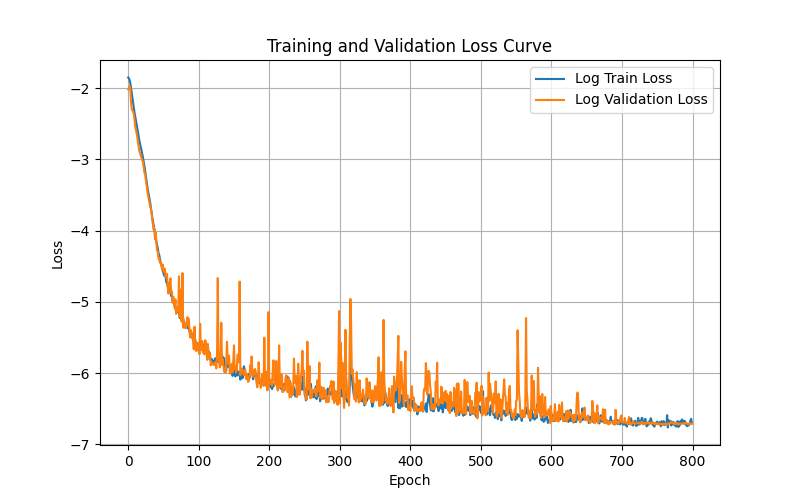
\includegraphics[width=\linewidth]{../assets/Training Loss and Validation Loss.png}
  \caption{Training Loss and Validation Loss}
\end{figure}

In the figure 4, figure 5, and figure 6 below, there are some example testing images before and after deep
learning reconstruction. Here we only show half of the output we obtained, the complete outcome
can be seen in the folder named /texttt{images}.
\begin{figure}[ht]
  \centering
  \begin{subfigure}[b]{0.8\linewidth}
    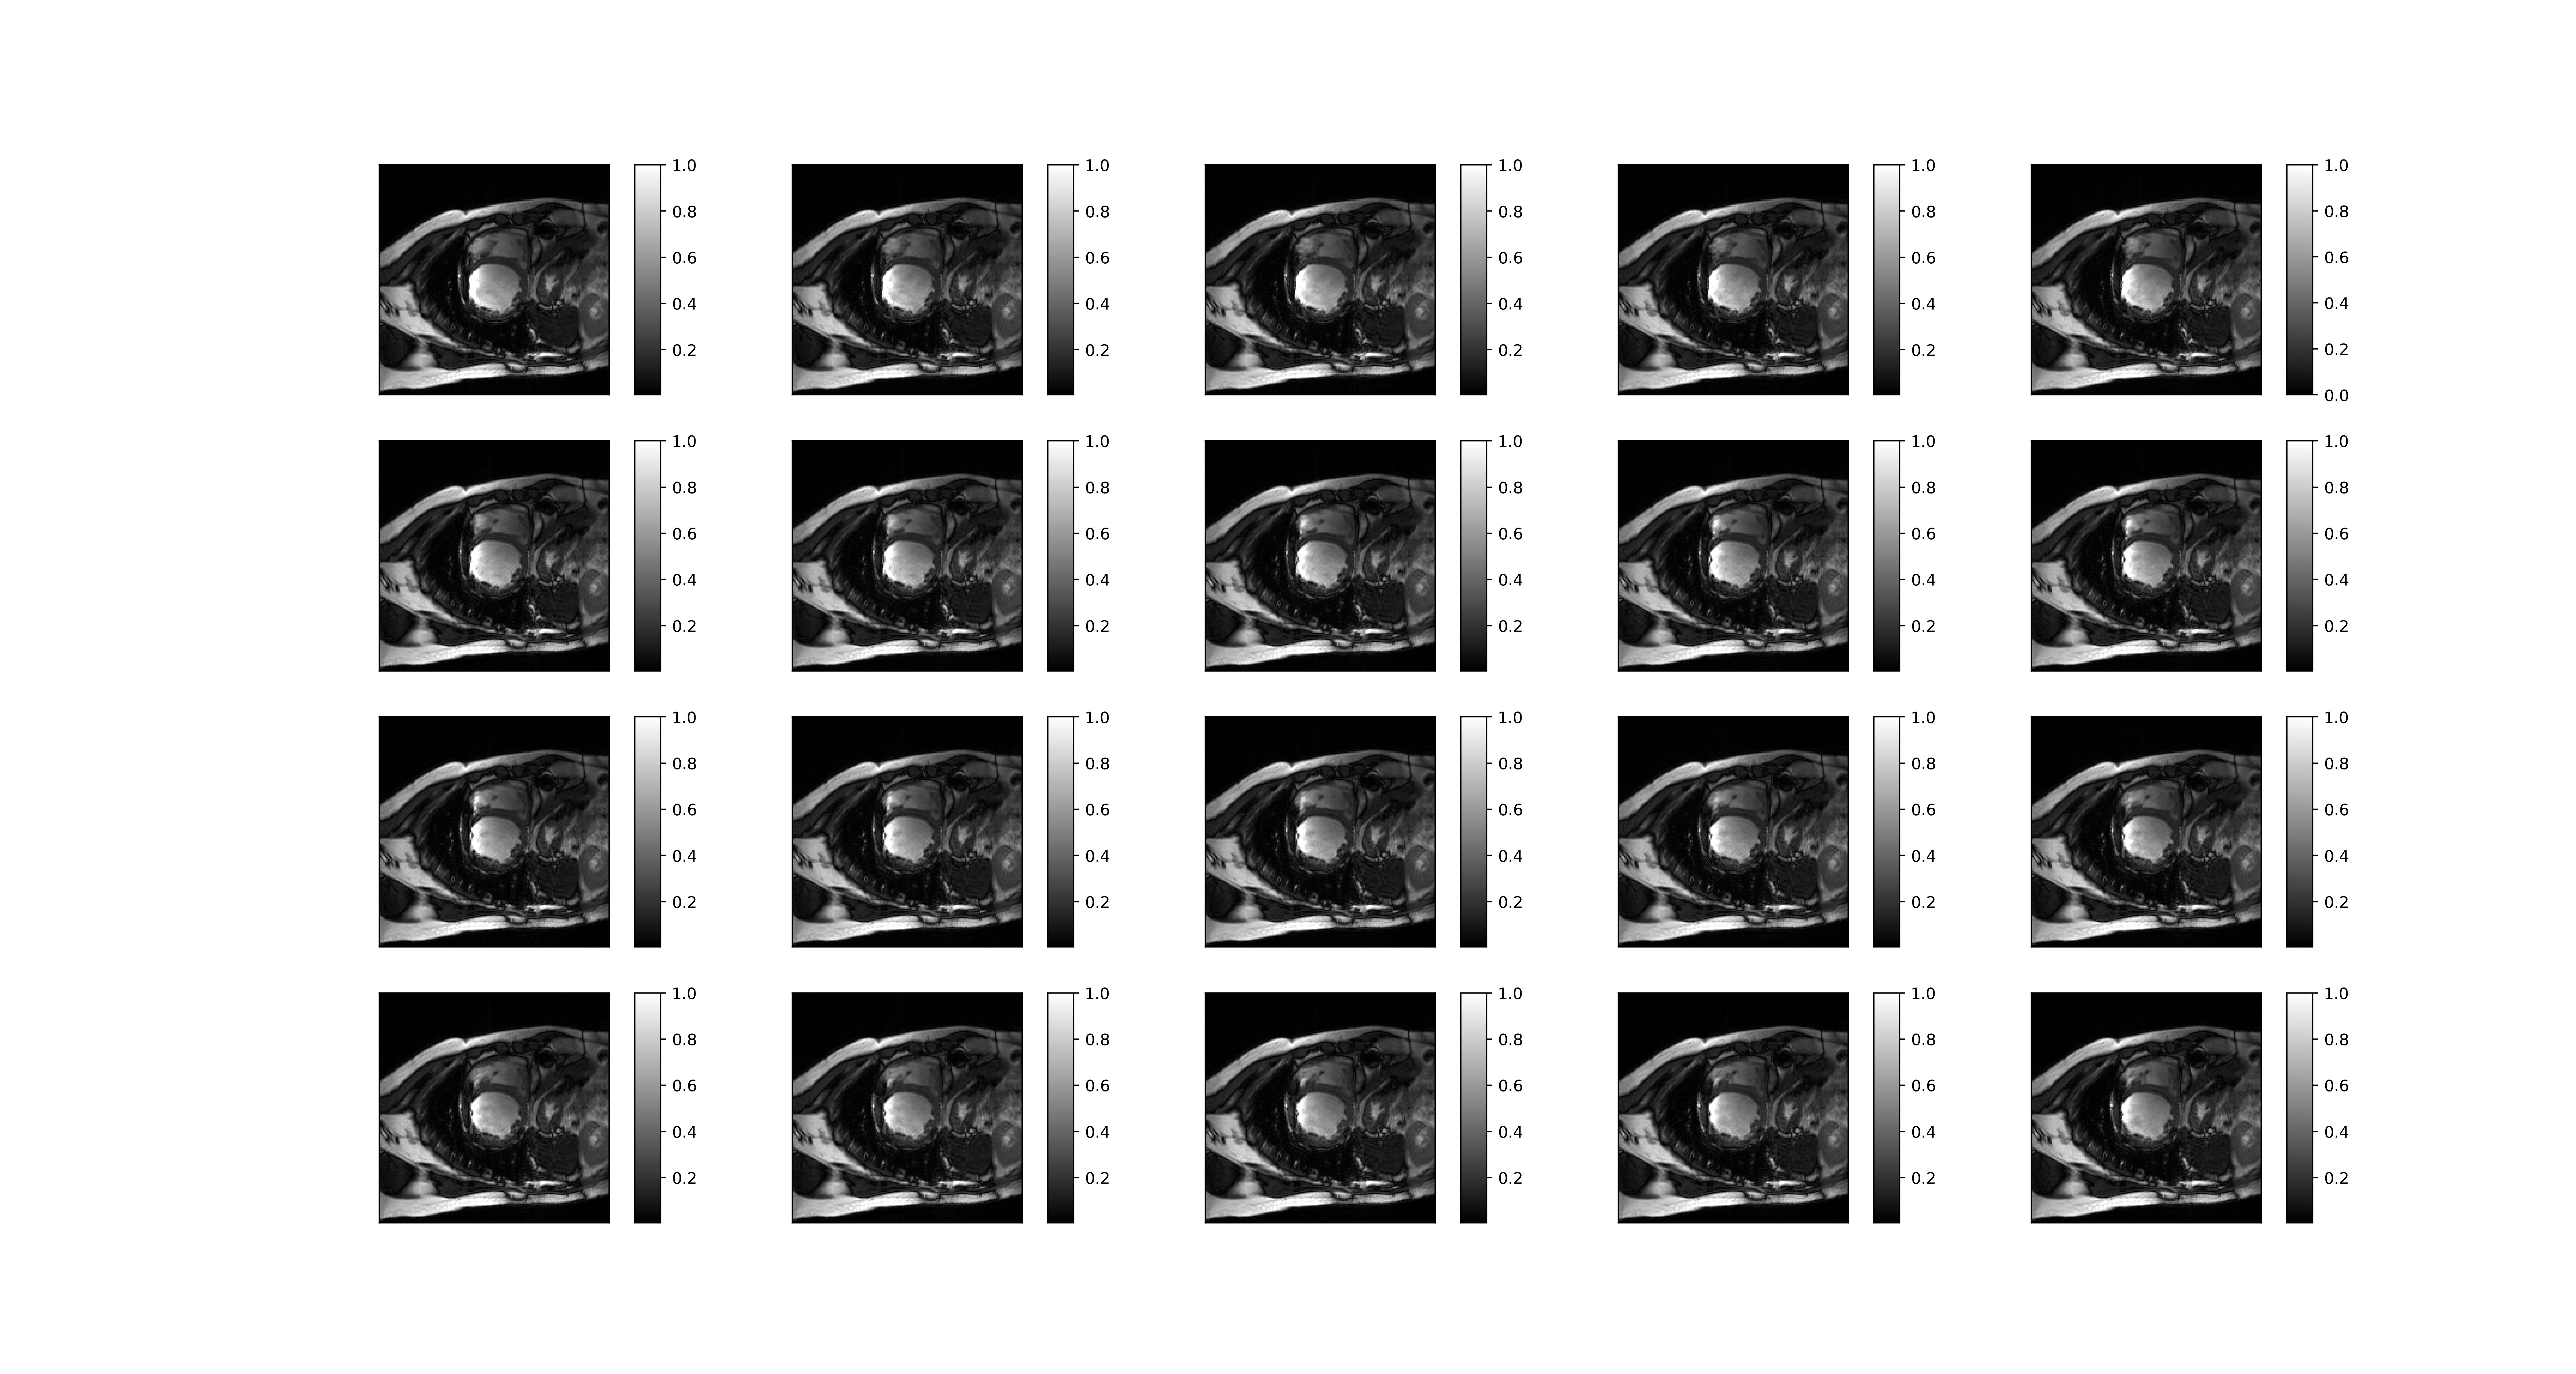
\includegraphics[width=\linewidth]{../images/output/full_sampling/full_sampling_0.png}
    \caption{fully sampled image 0}
  \end{subfigure}
  \quad
  \begin{subfigure}[b]{0.8\linewidth}
    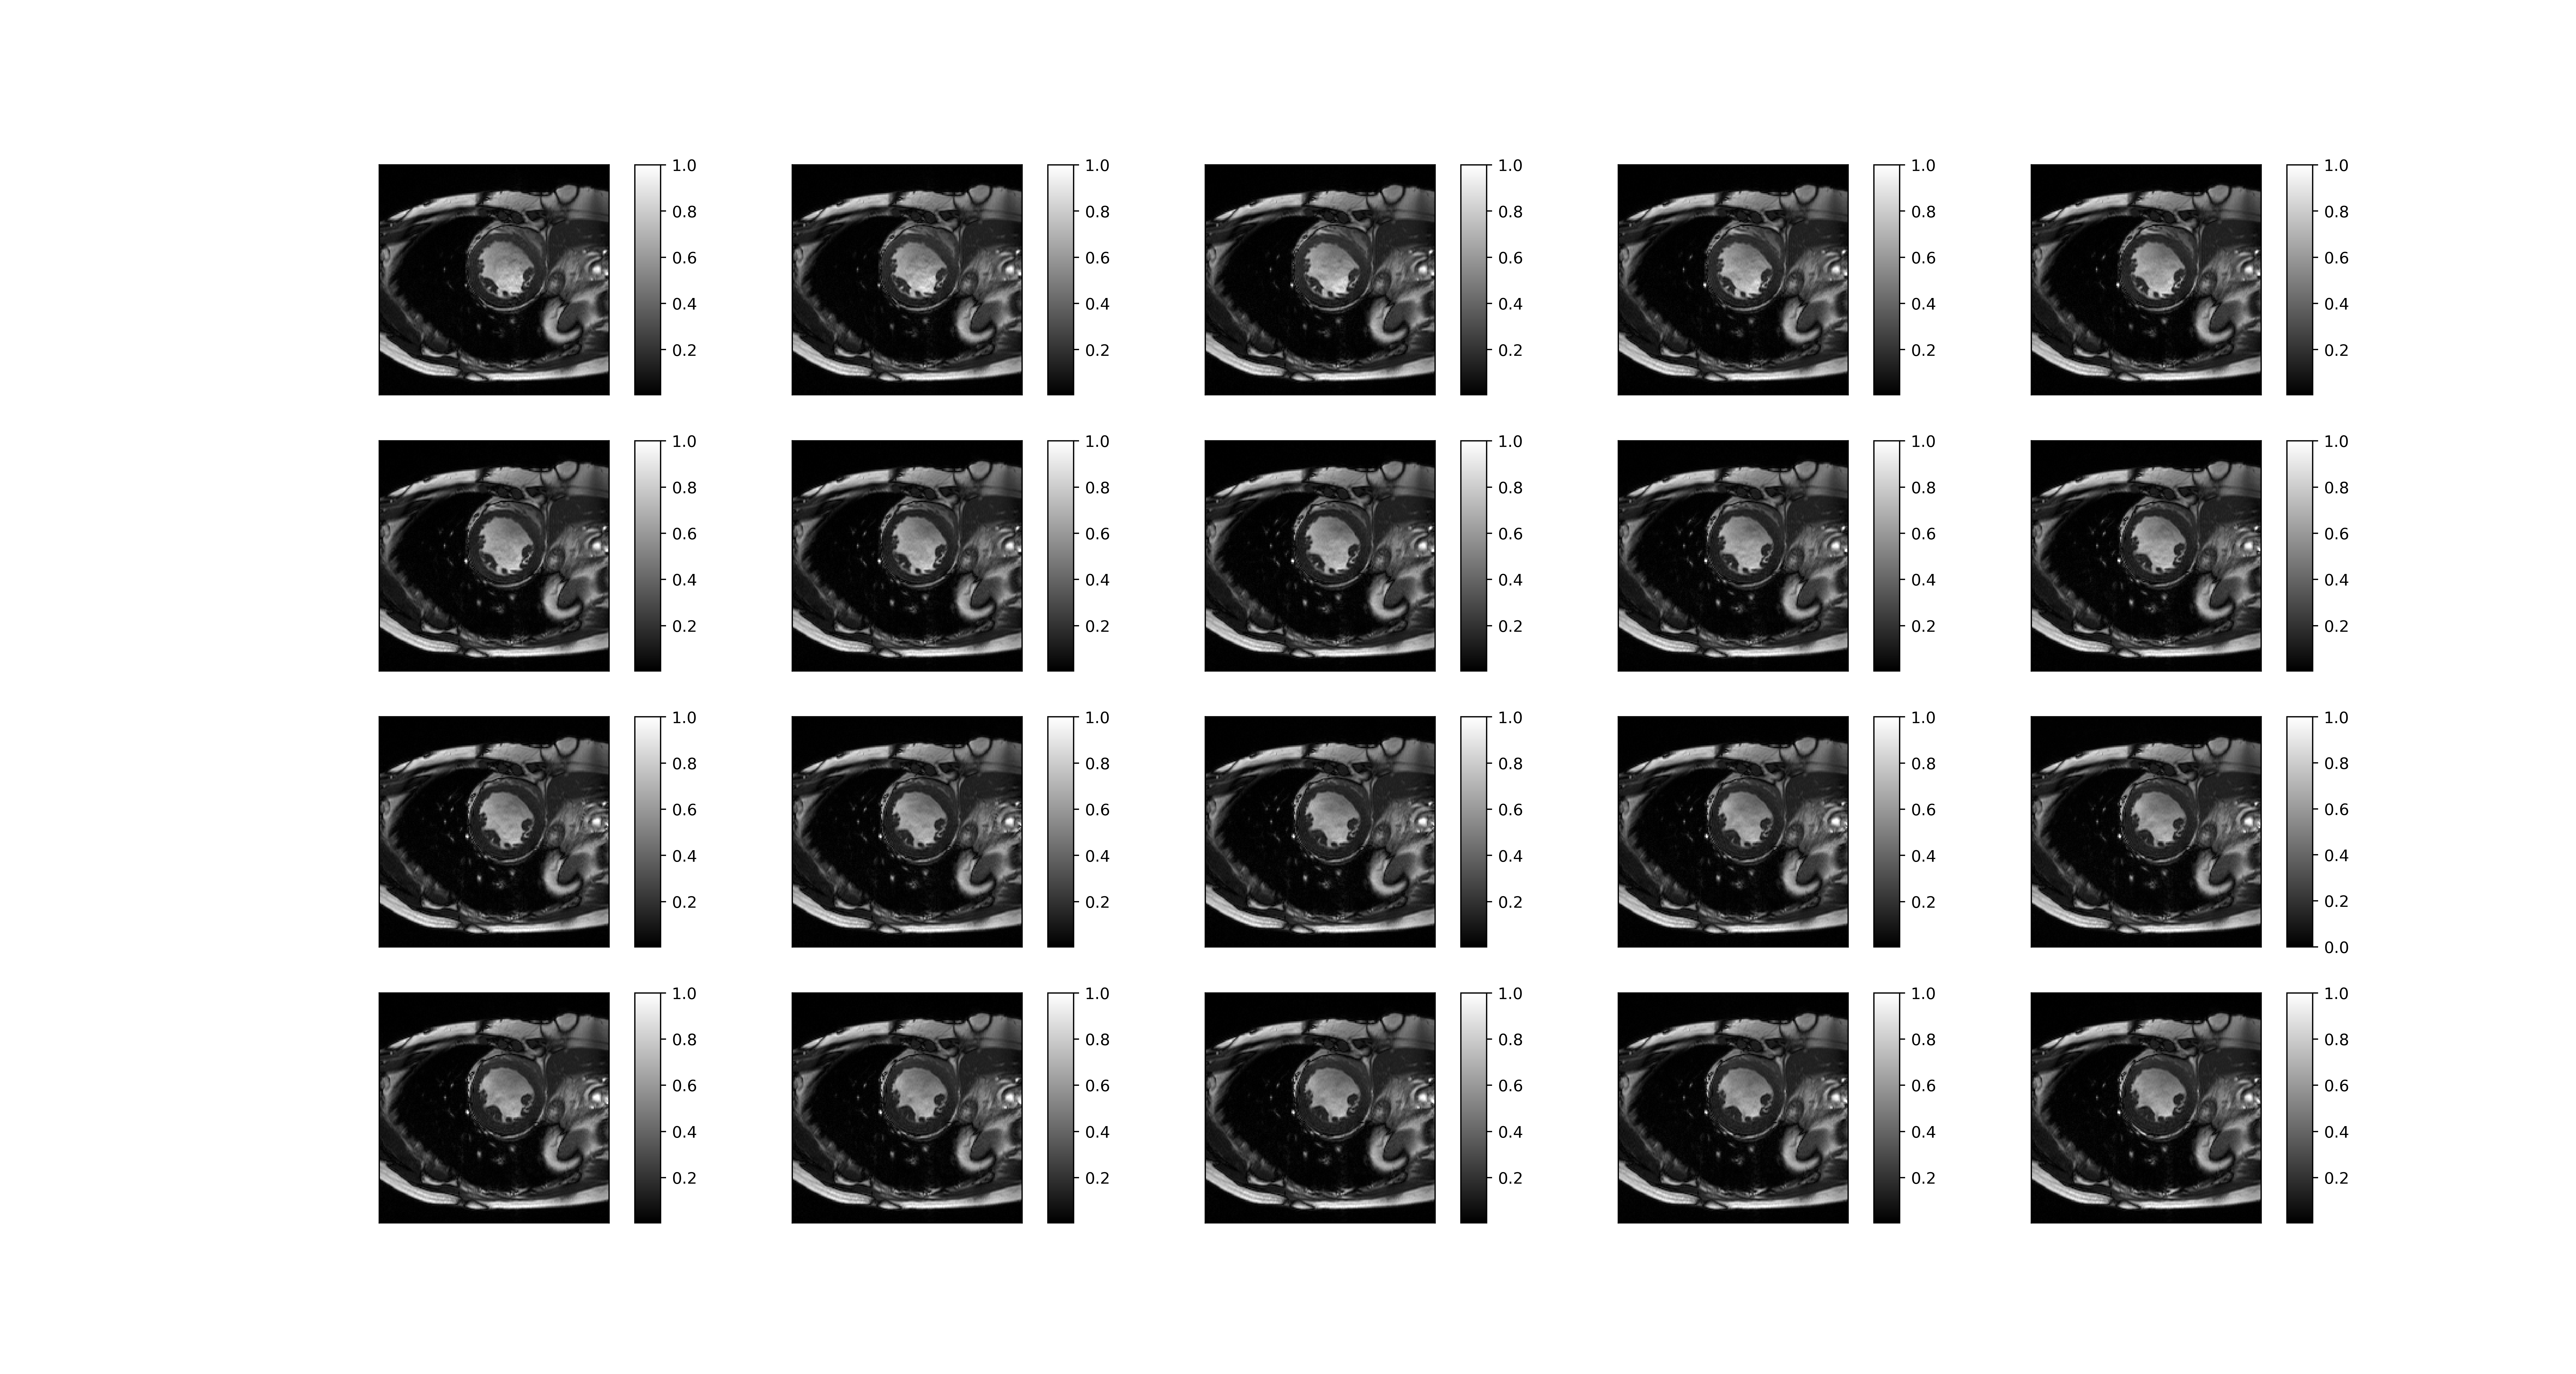
\includegraphics[width=\linewidth]{../images/output/full_sampling/full_sampling_1.png}
    \caption{fully sampled image 1}
  \end{subfigure}
  \quad
  \begin{subfigure}[b]{0.8\linewidth}
    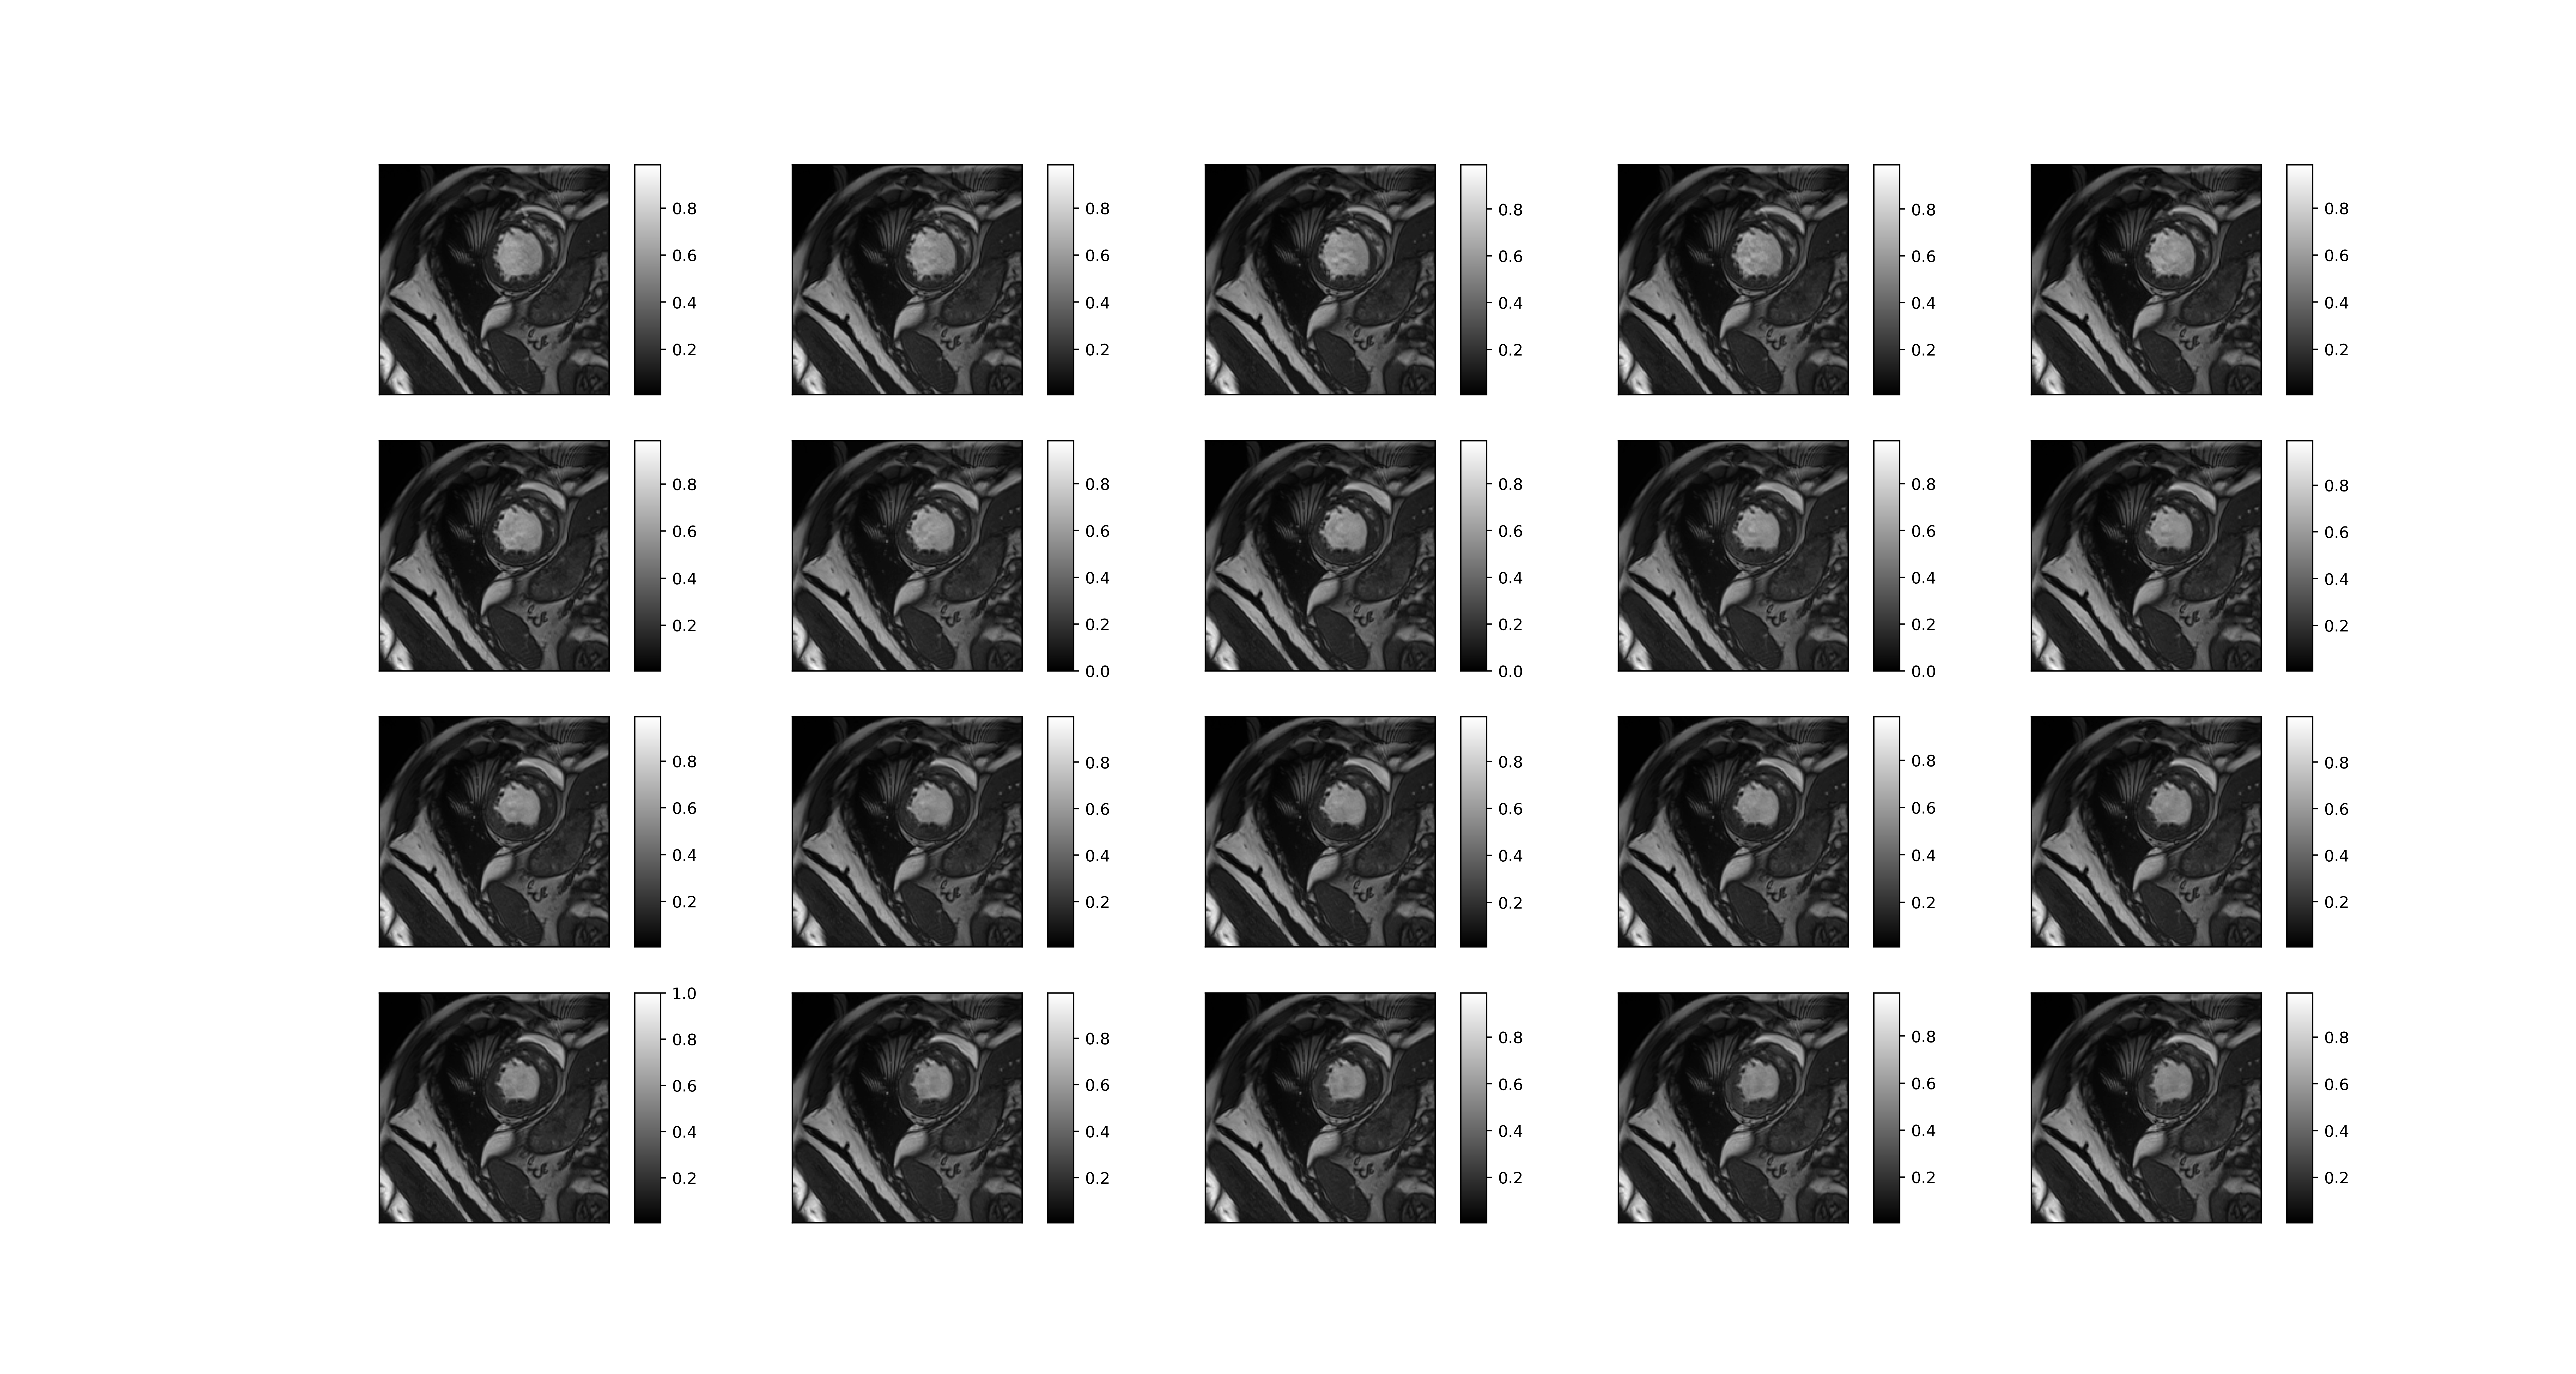
\includegraphics[width=\linewidth]{../images/output/full_sampling/full_sampling_2.png}
    \caption{fully sampled image 2}
  \end{subfigure}
  \caption{Fully Sampled Images (Ground Truth)}
\end{figure}

\begin{figure}[ht]
  \centering
  \begin{subfigure}[b]{0.8\linewidth}
    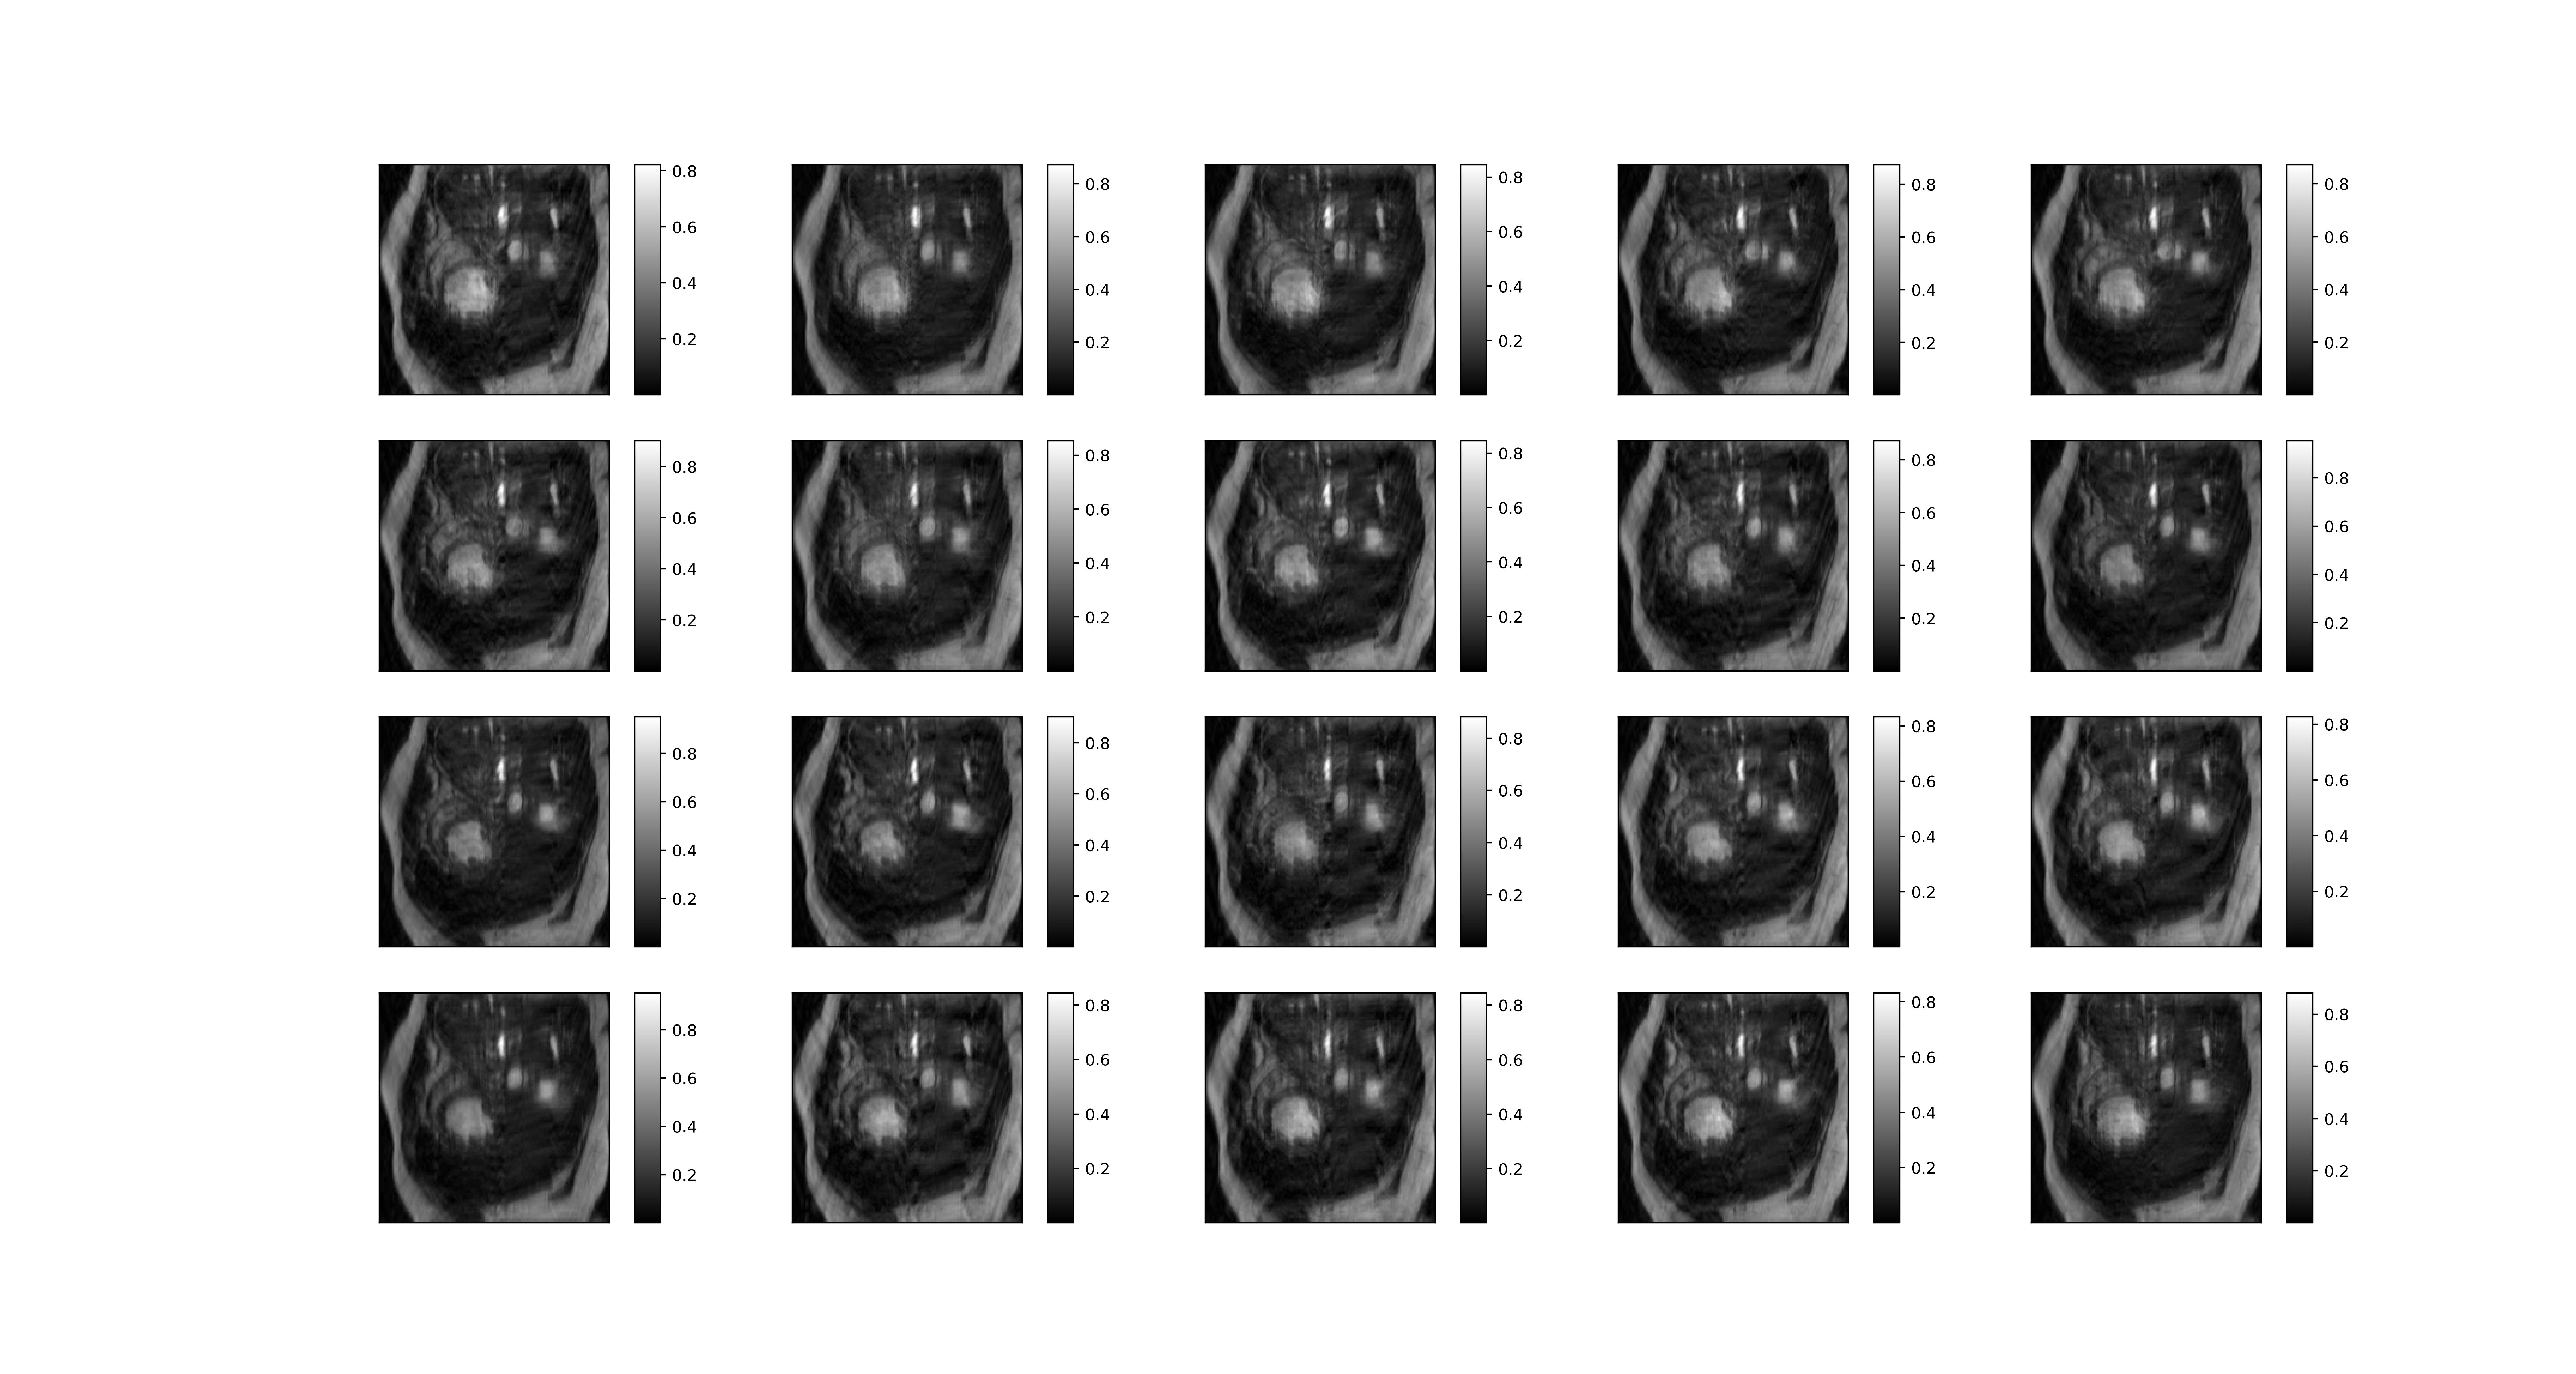
\includegraphics[width=\linewidth]{../images/output/under_sampling/under_sampling_0.png}
    \caption{under sampled image 0}
  \end{subfigure}
  \quad
  \begin{subfigure}[b]{0.8\linewidth}
    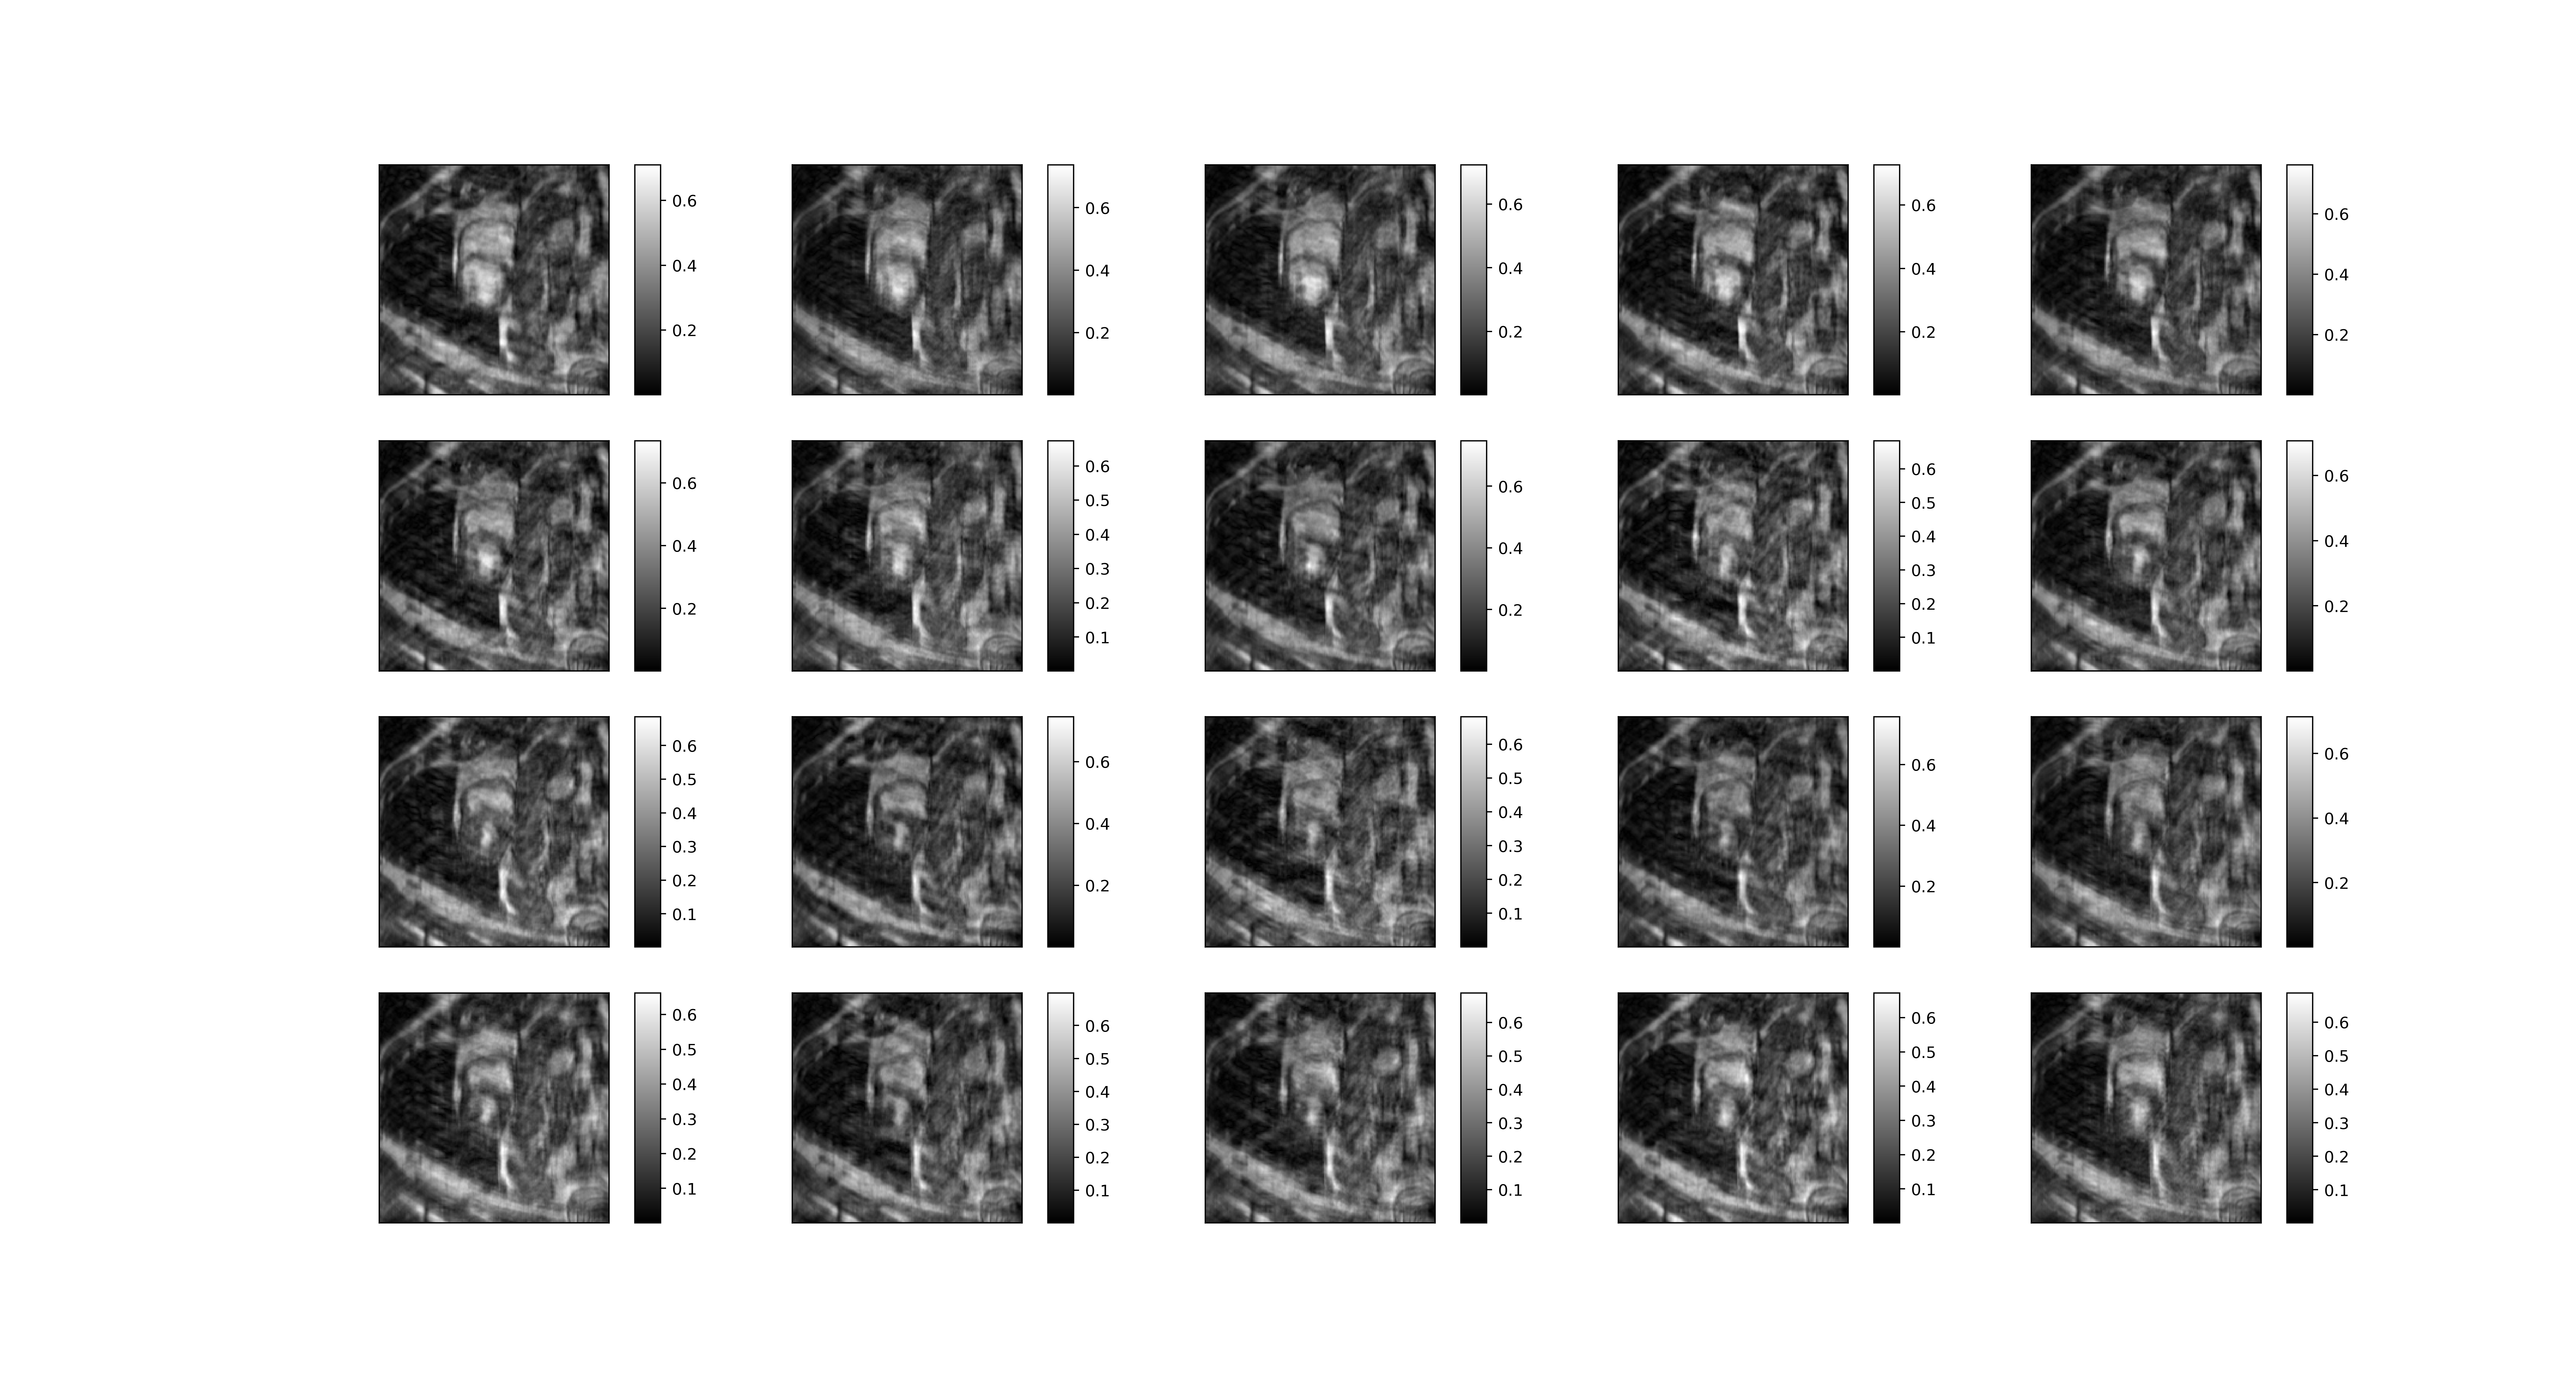
\includegraphics[width=\linewidth]{../images/output/under_sampling/under_sampling_1.png}
    \caption{under sampled image 1}
  \end{subfigure}
  \quad
  \begin{subfigure}[b]{0.8\linewidth}
    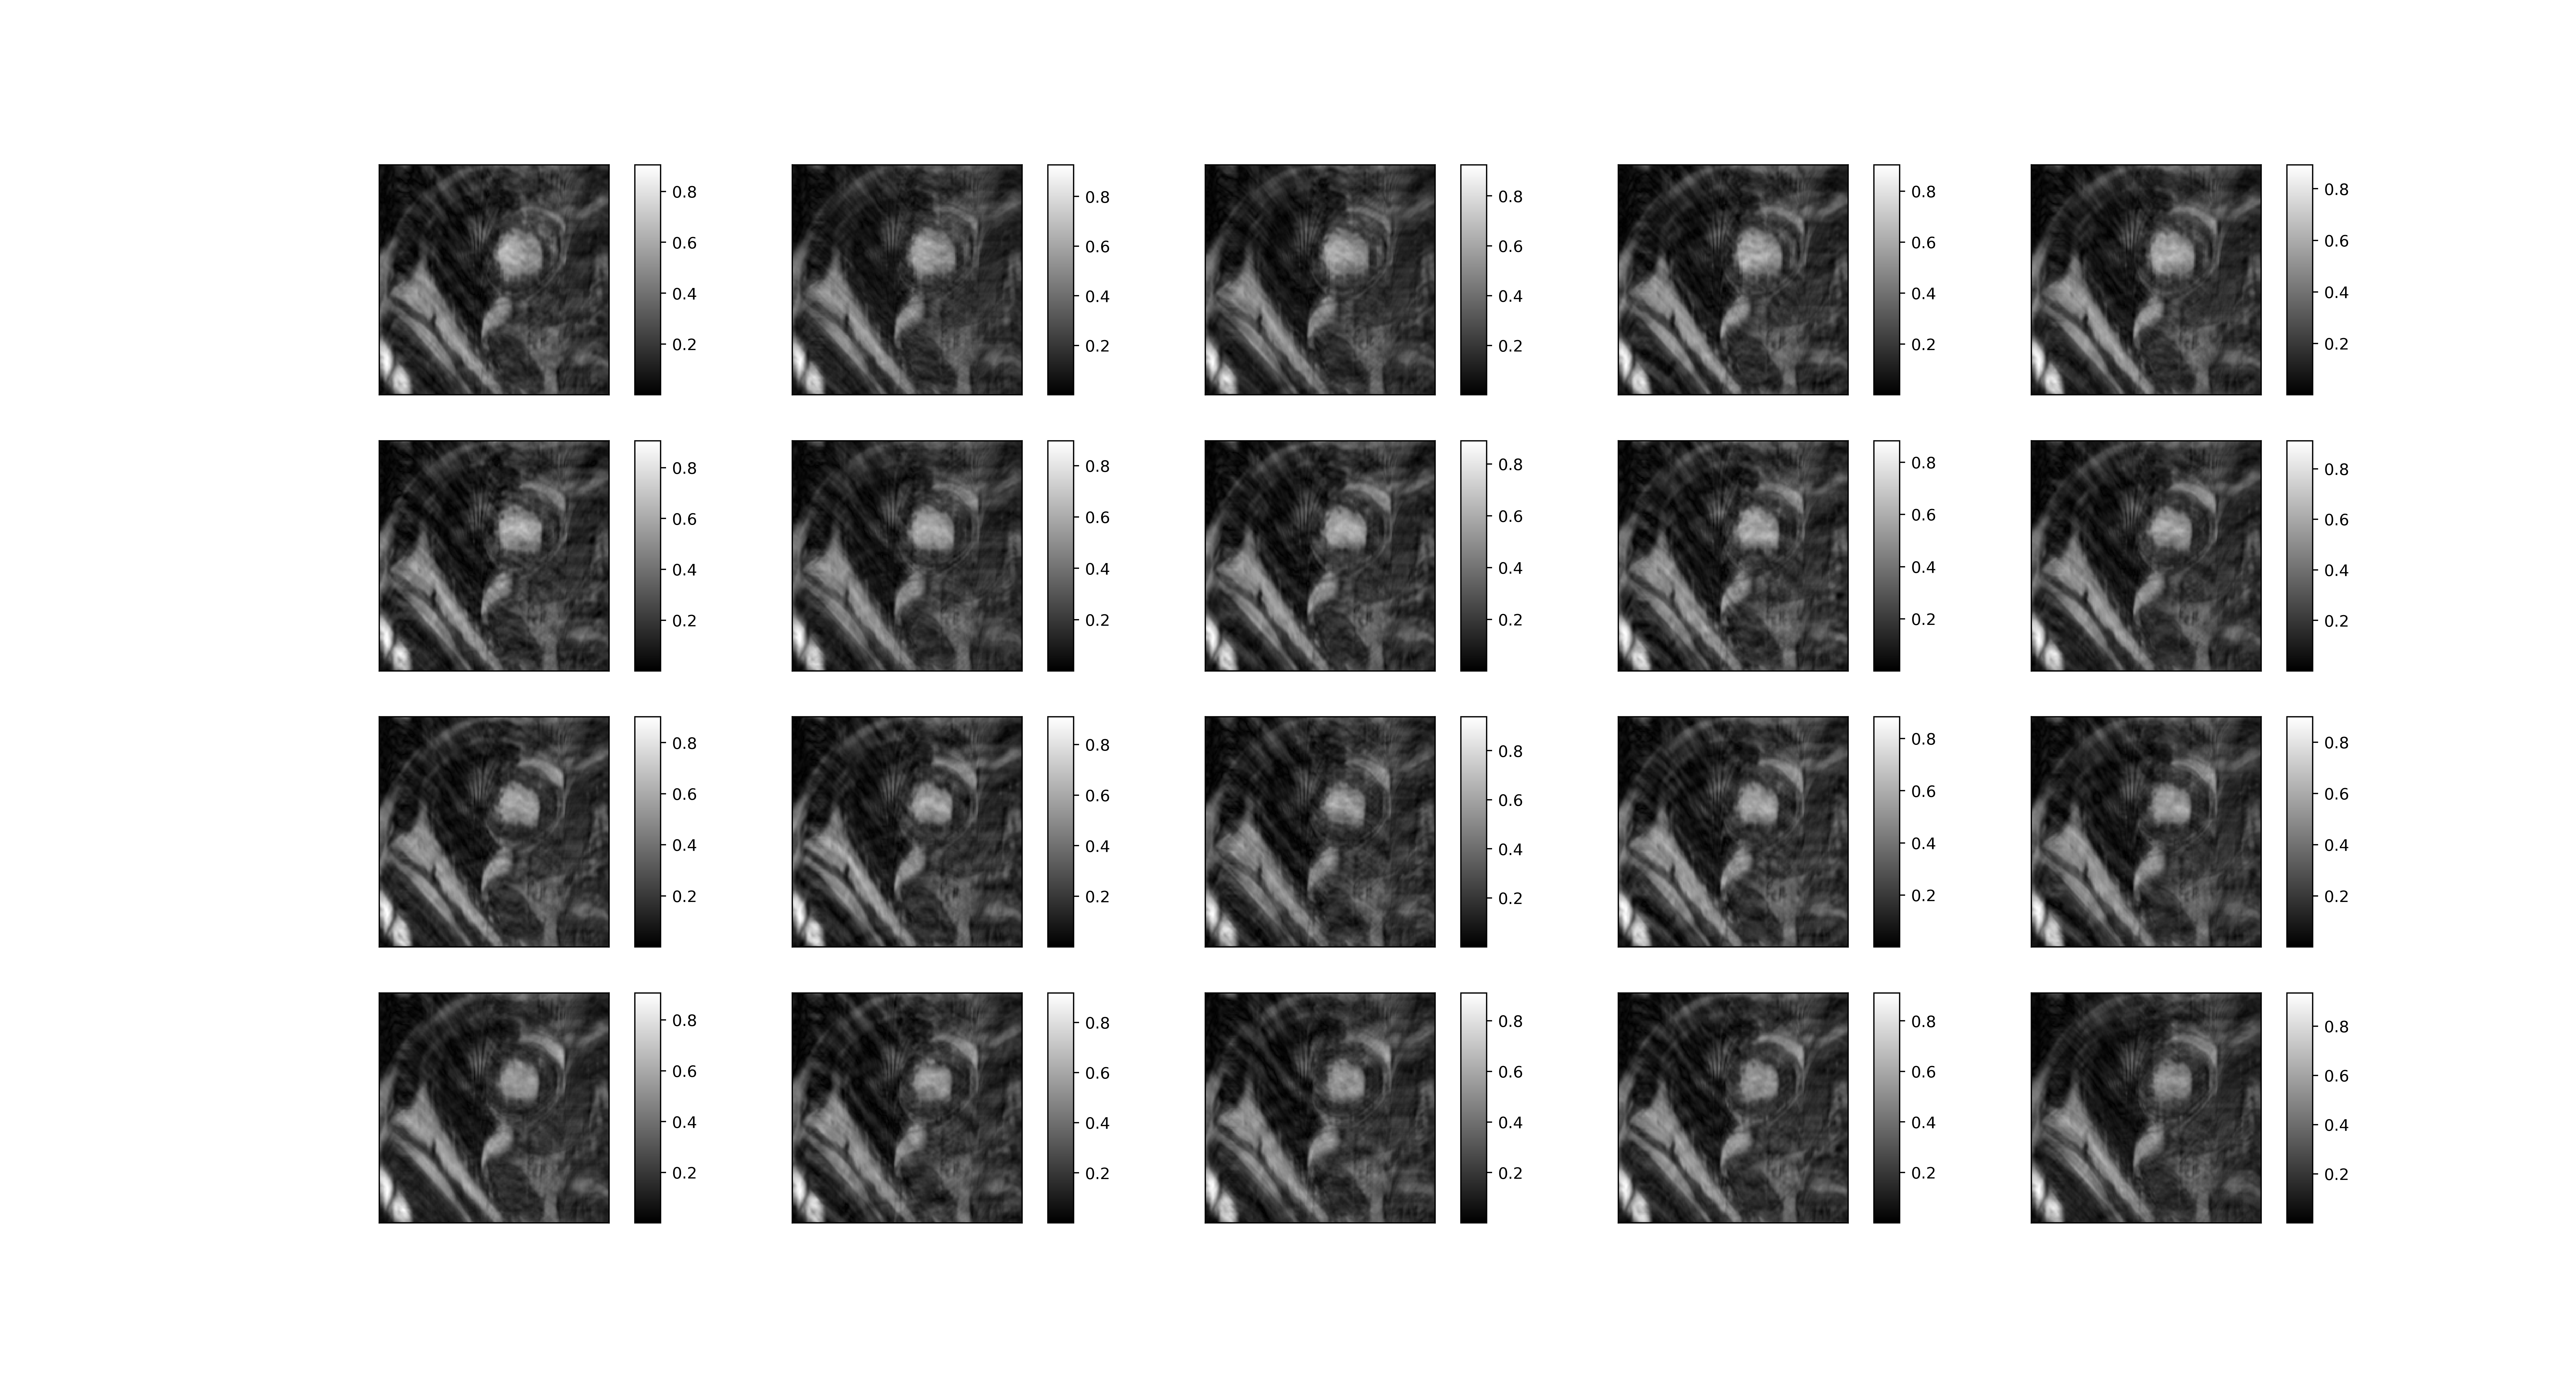
\includegraphics[width=\linewidth]{../images/output/under_sampling/under_sampling_2.png}
    \caption{under sampled image 2}
  \end{subfigure}
  \caption{Under Sampled Images}
\end{figure}

\begin{figure}[ht]
  \centering
  \begin{subfigure}[b]{0.8\linewidth}
    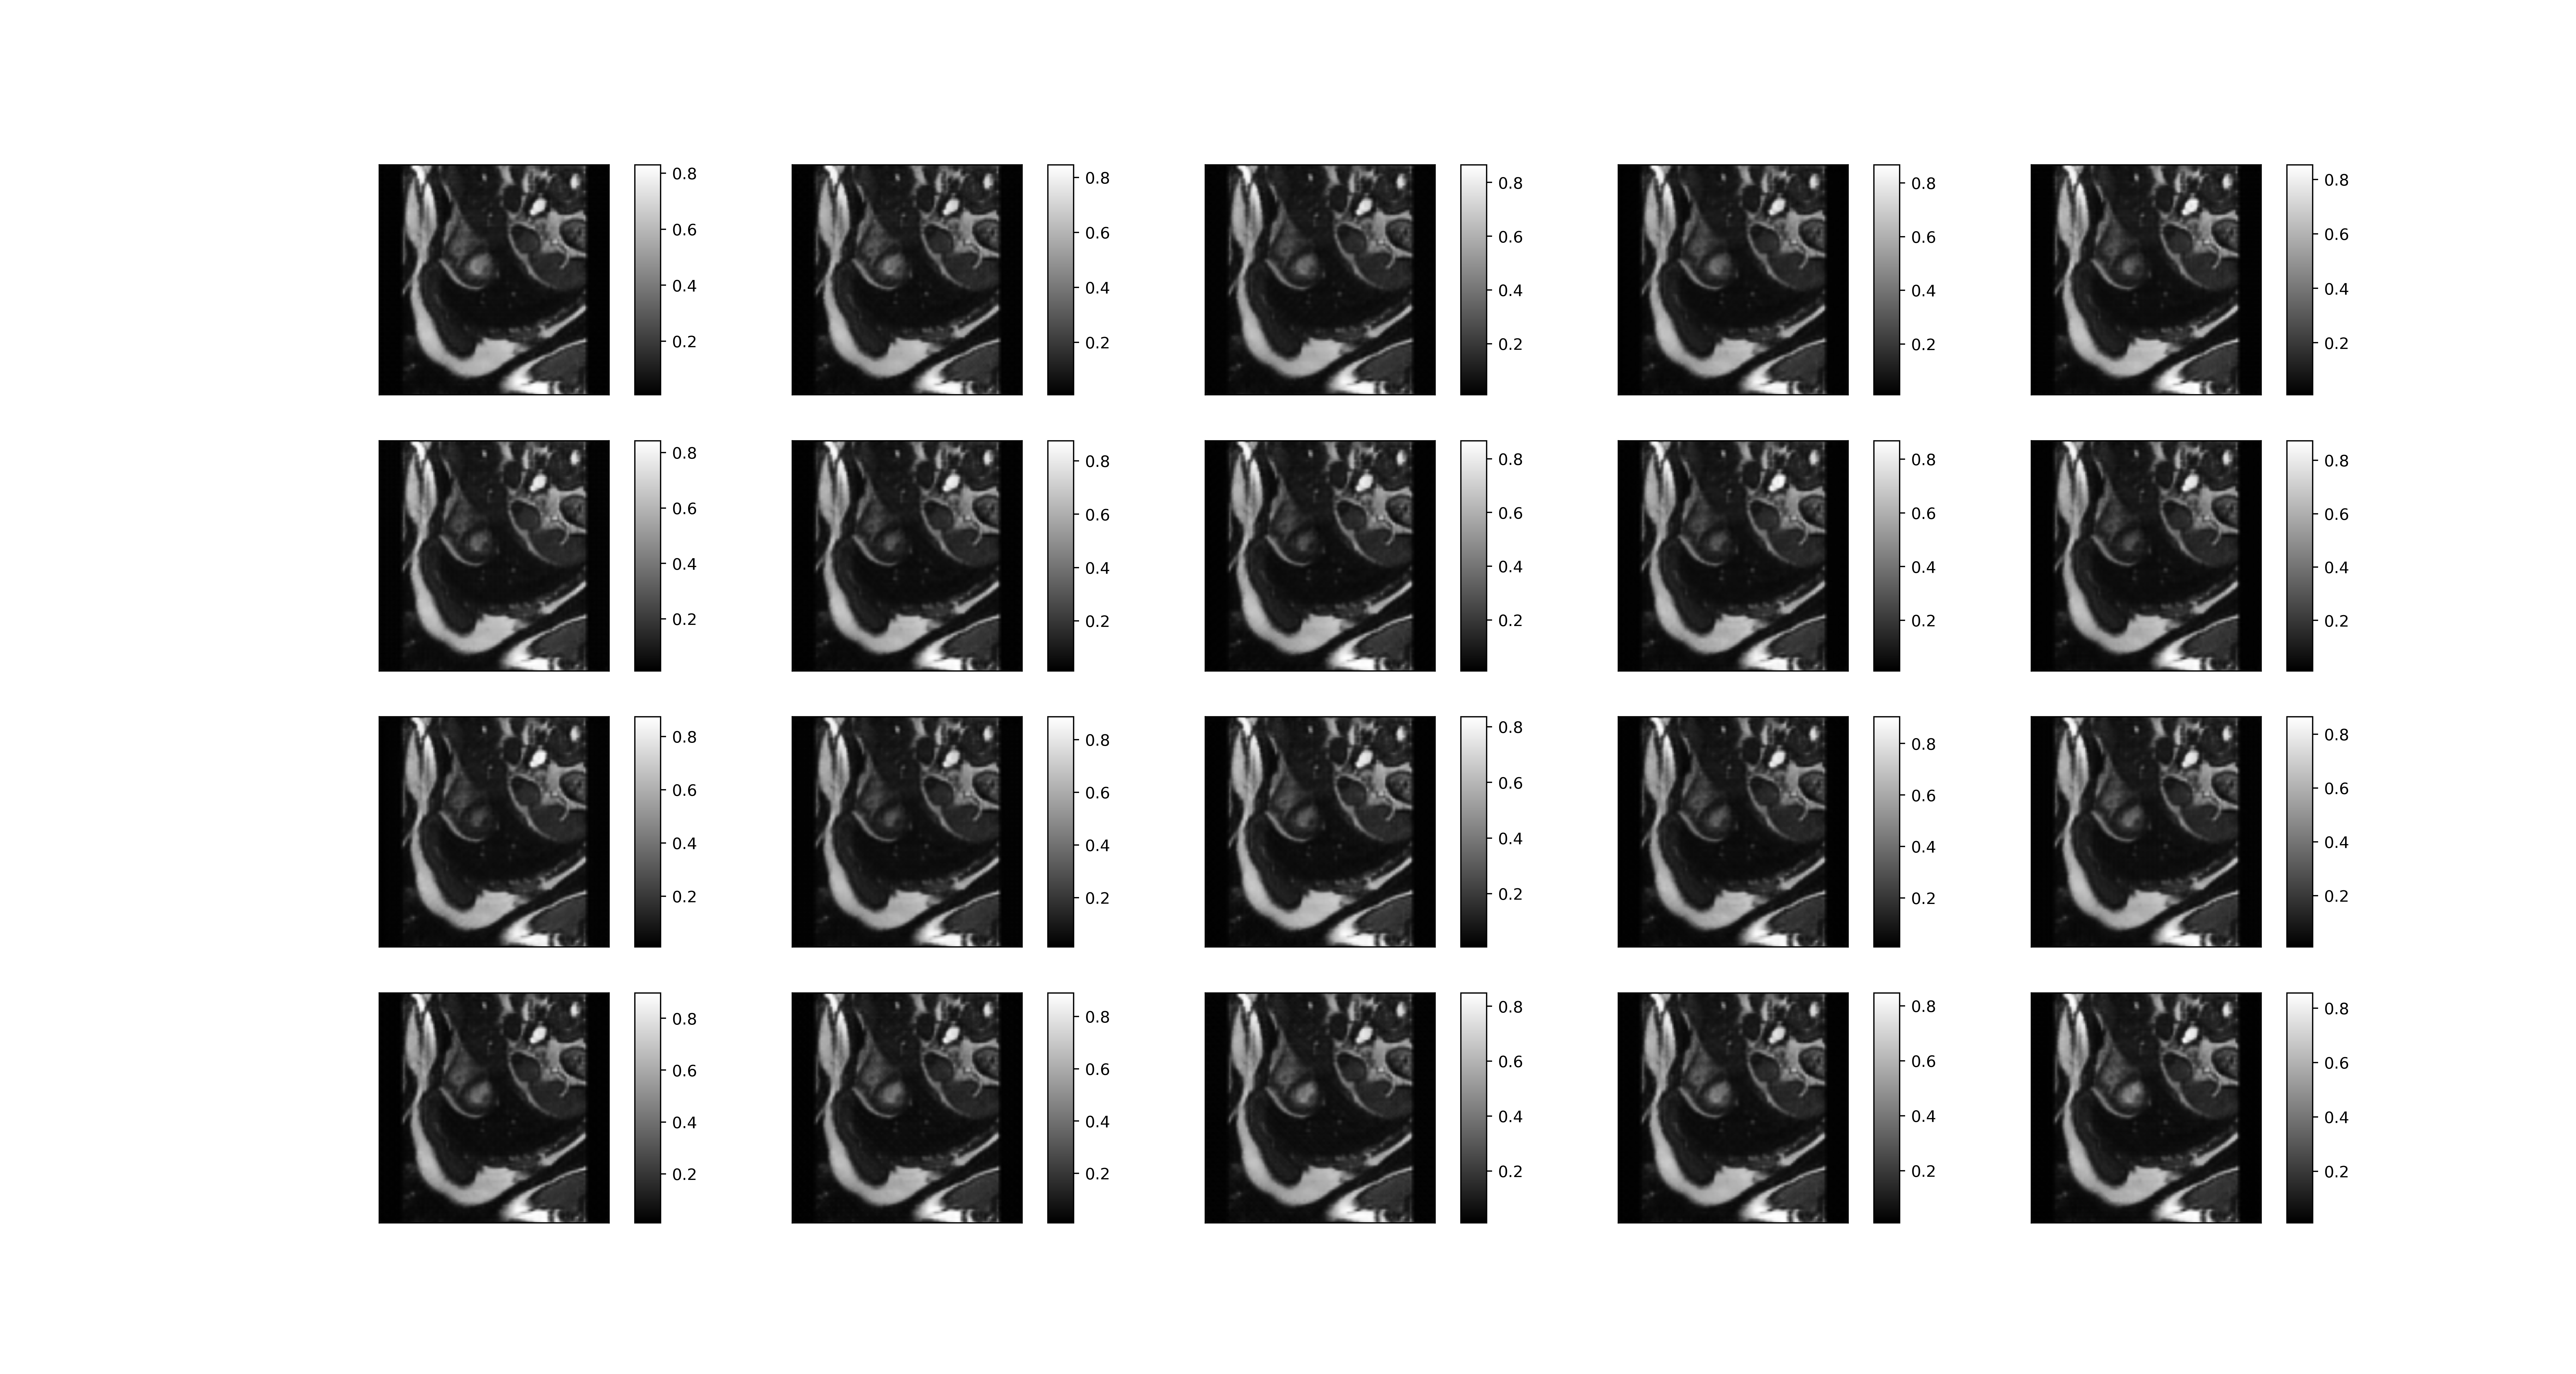
\includegraphics[width=\linewidth]{../images/output/reconstruction/reconstruction_0.png}
    \caption{reconstruction image 0}
  \end{subfigure}
  \quad
  \begin{subfigure}[b]{0.8\linewidth}
    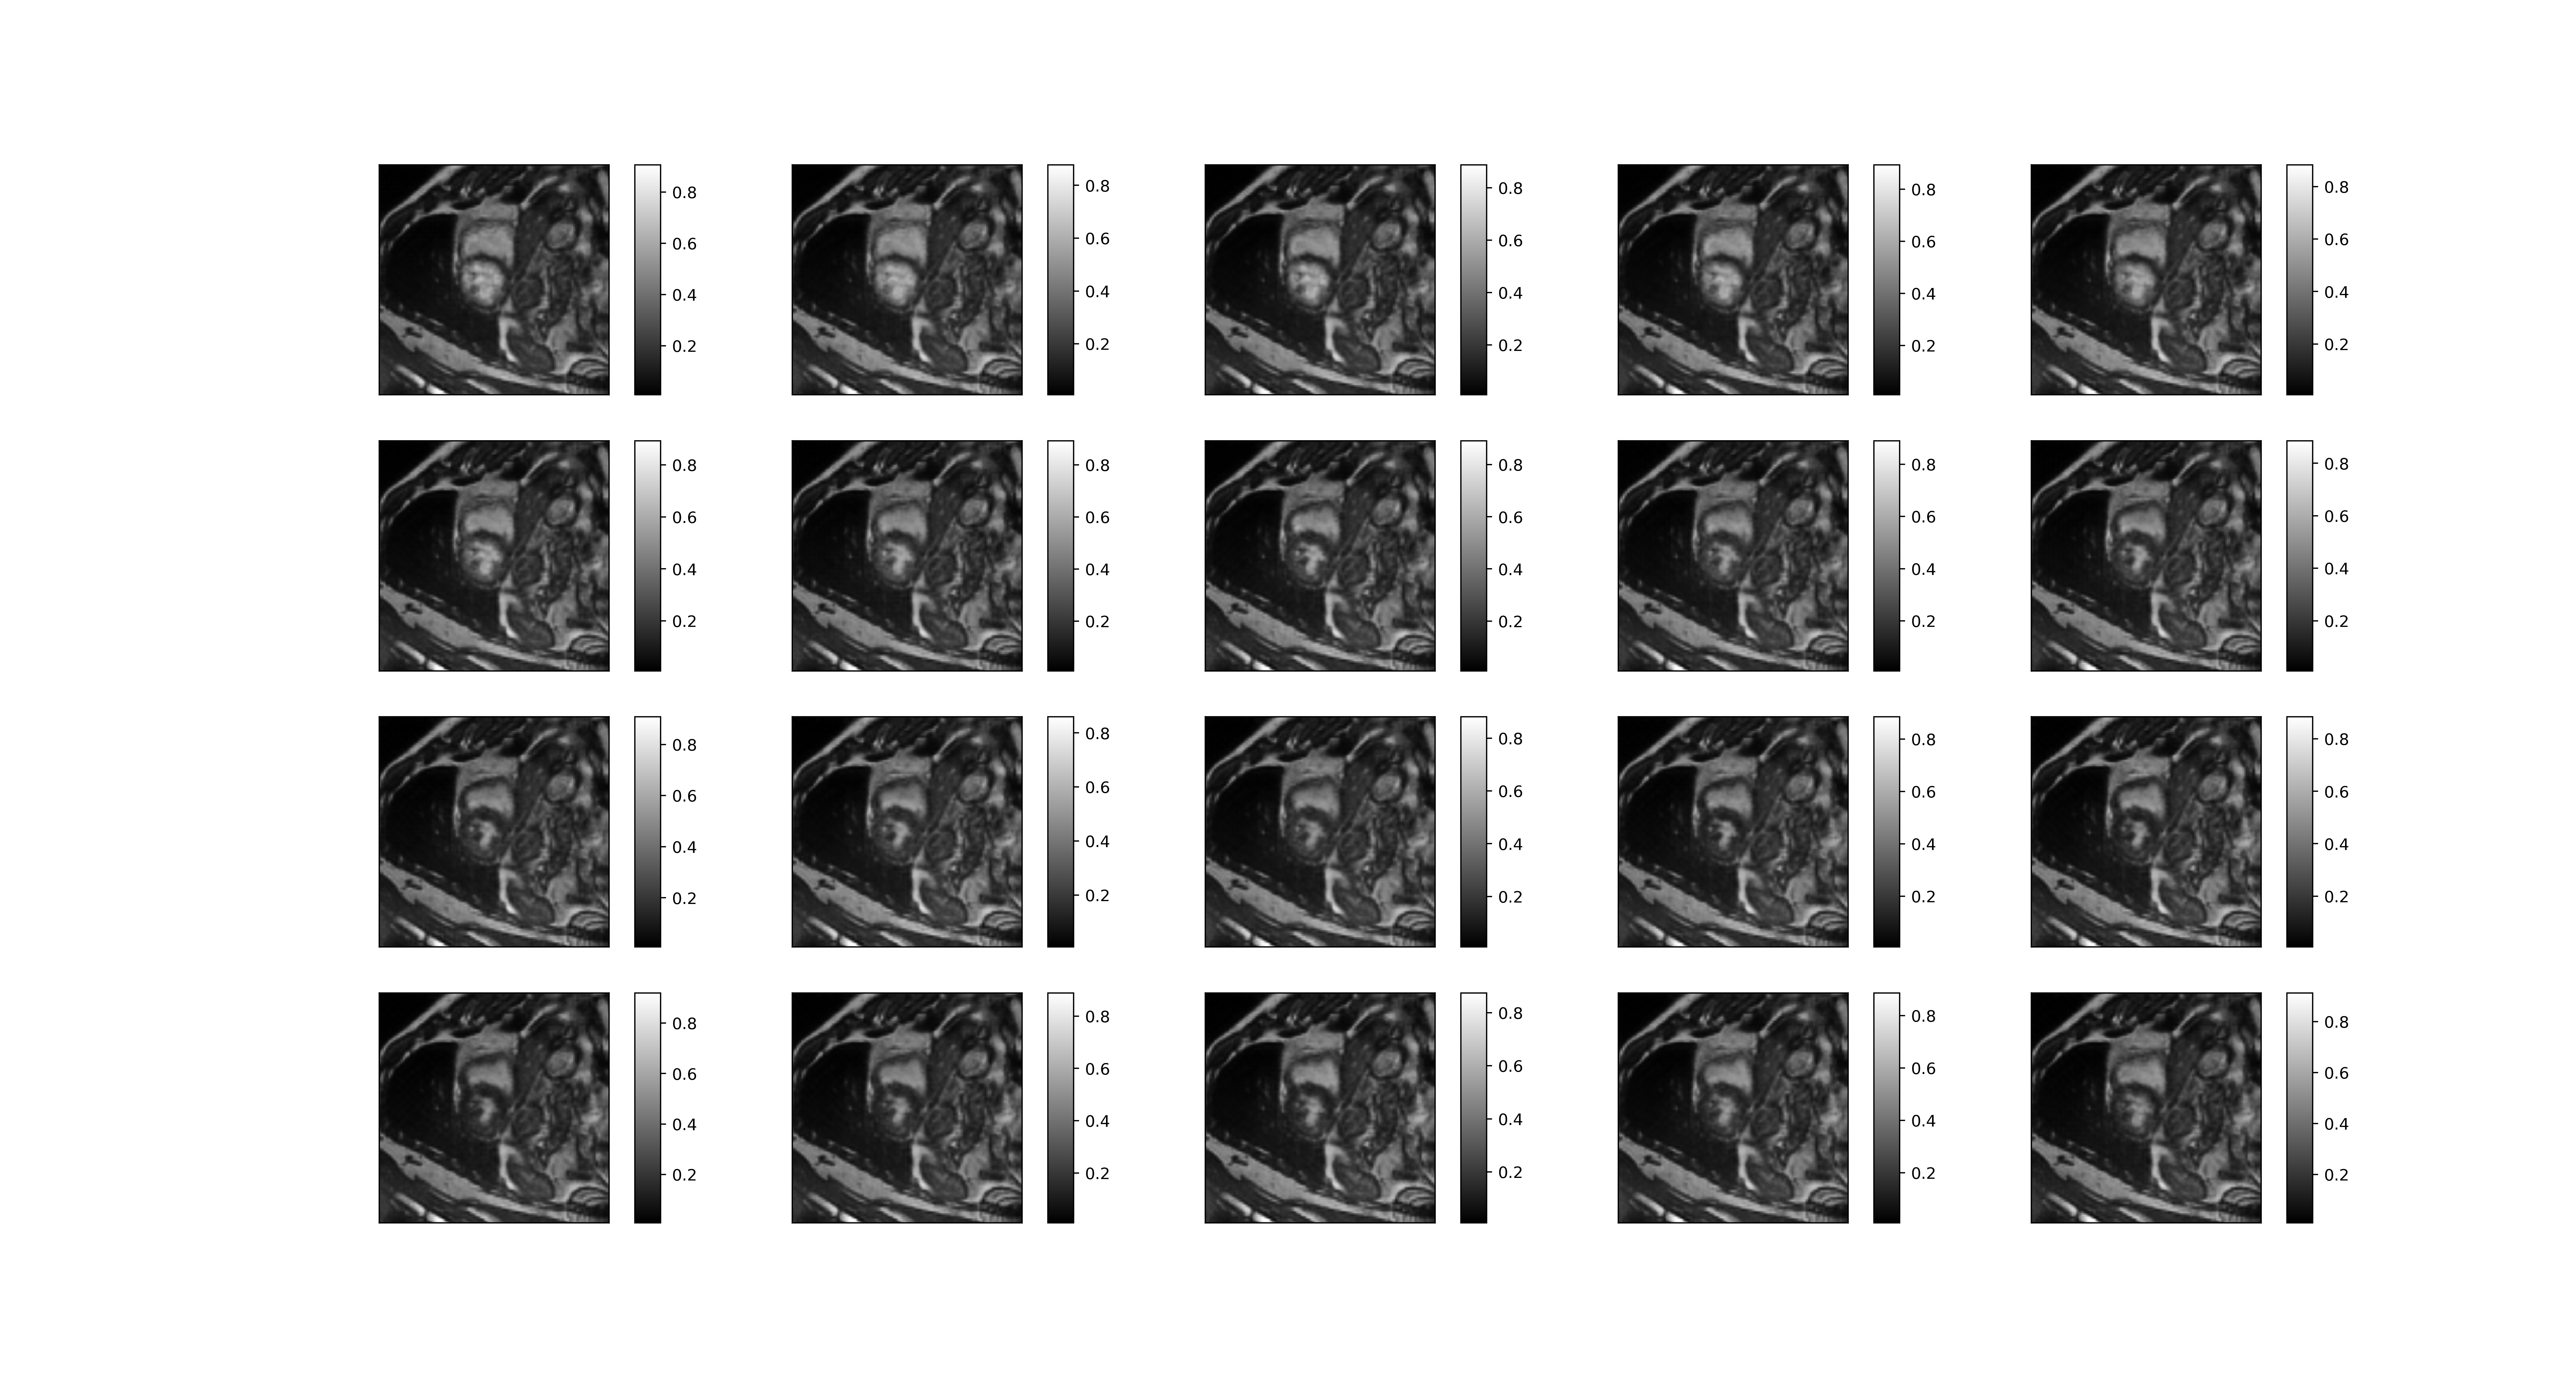
\includegraphics[width=\linewidth]{../images/output/reconstruction/reconstruction_1.png}
    \caption{reconstruction image 1}
  \end{subfigure}
  \quad
  \begin{subfigure}[b]{0.8\linewidth}
    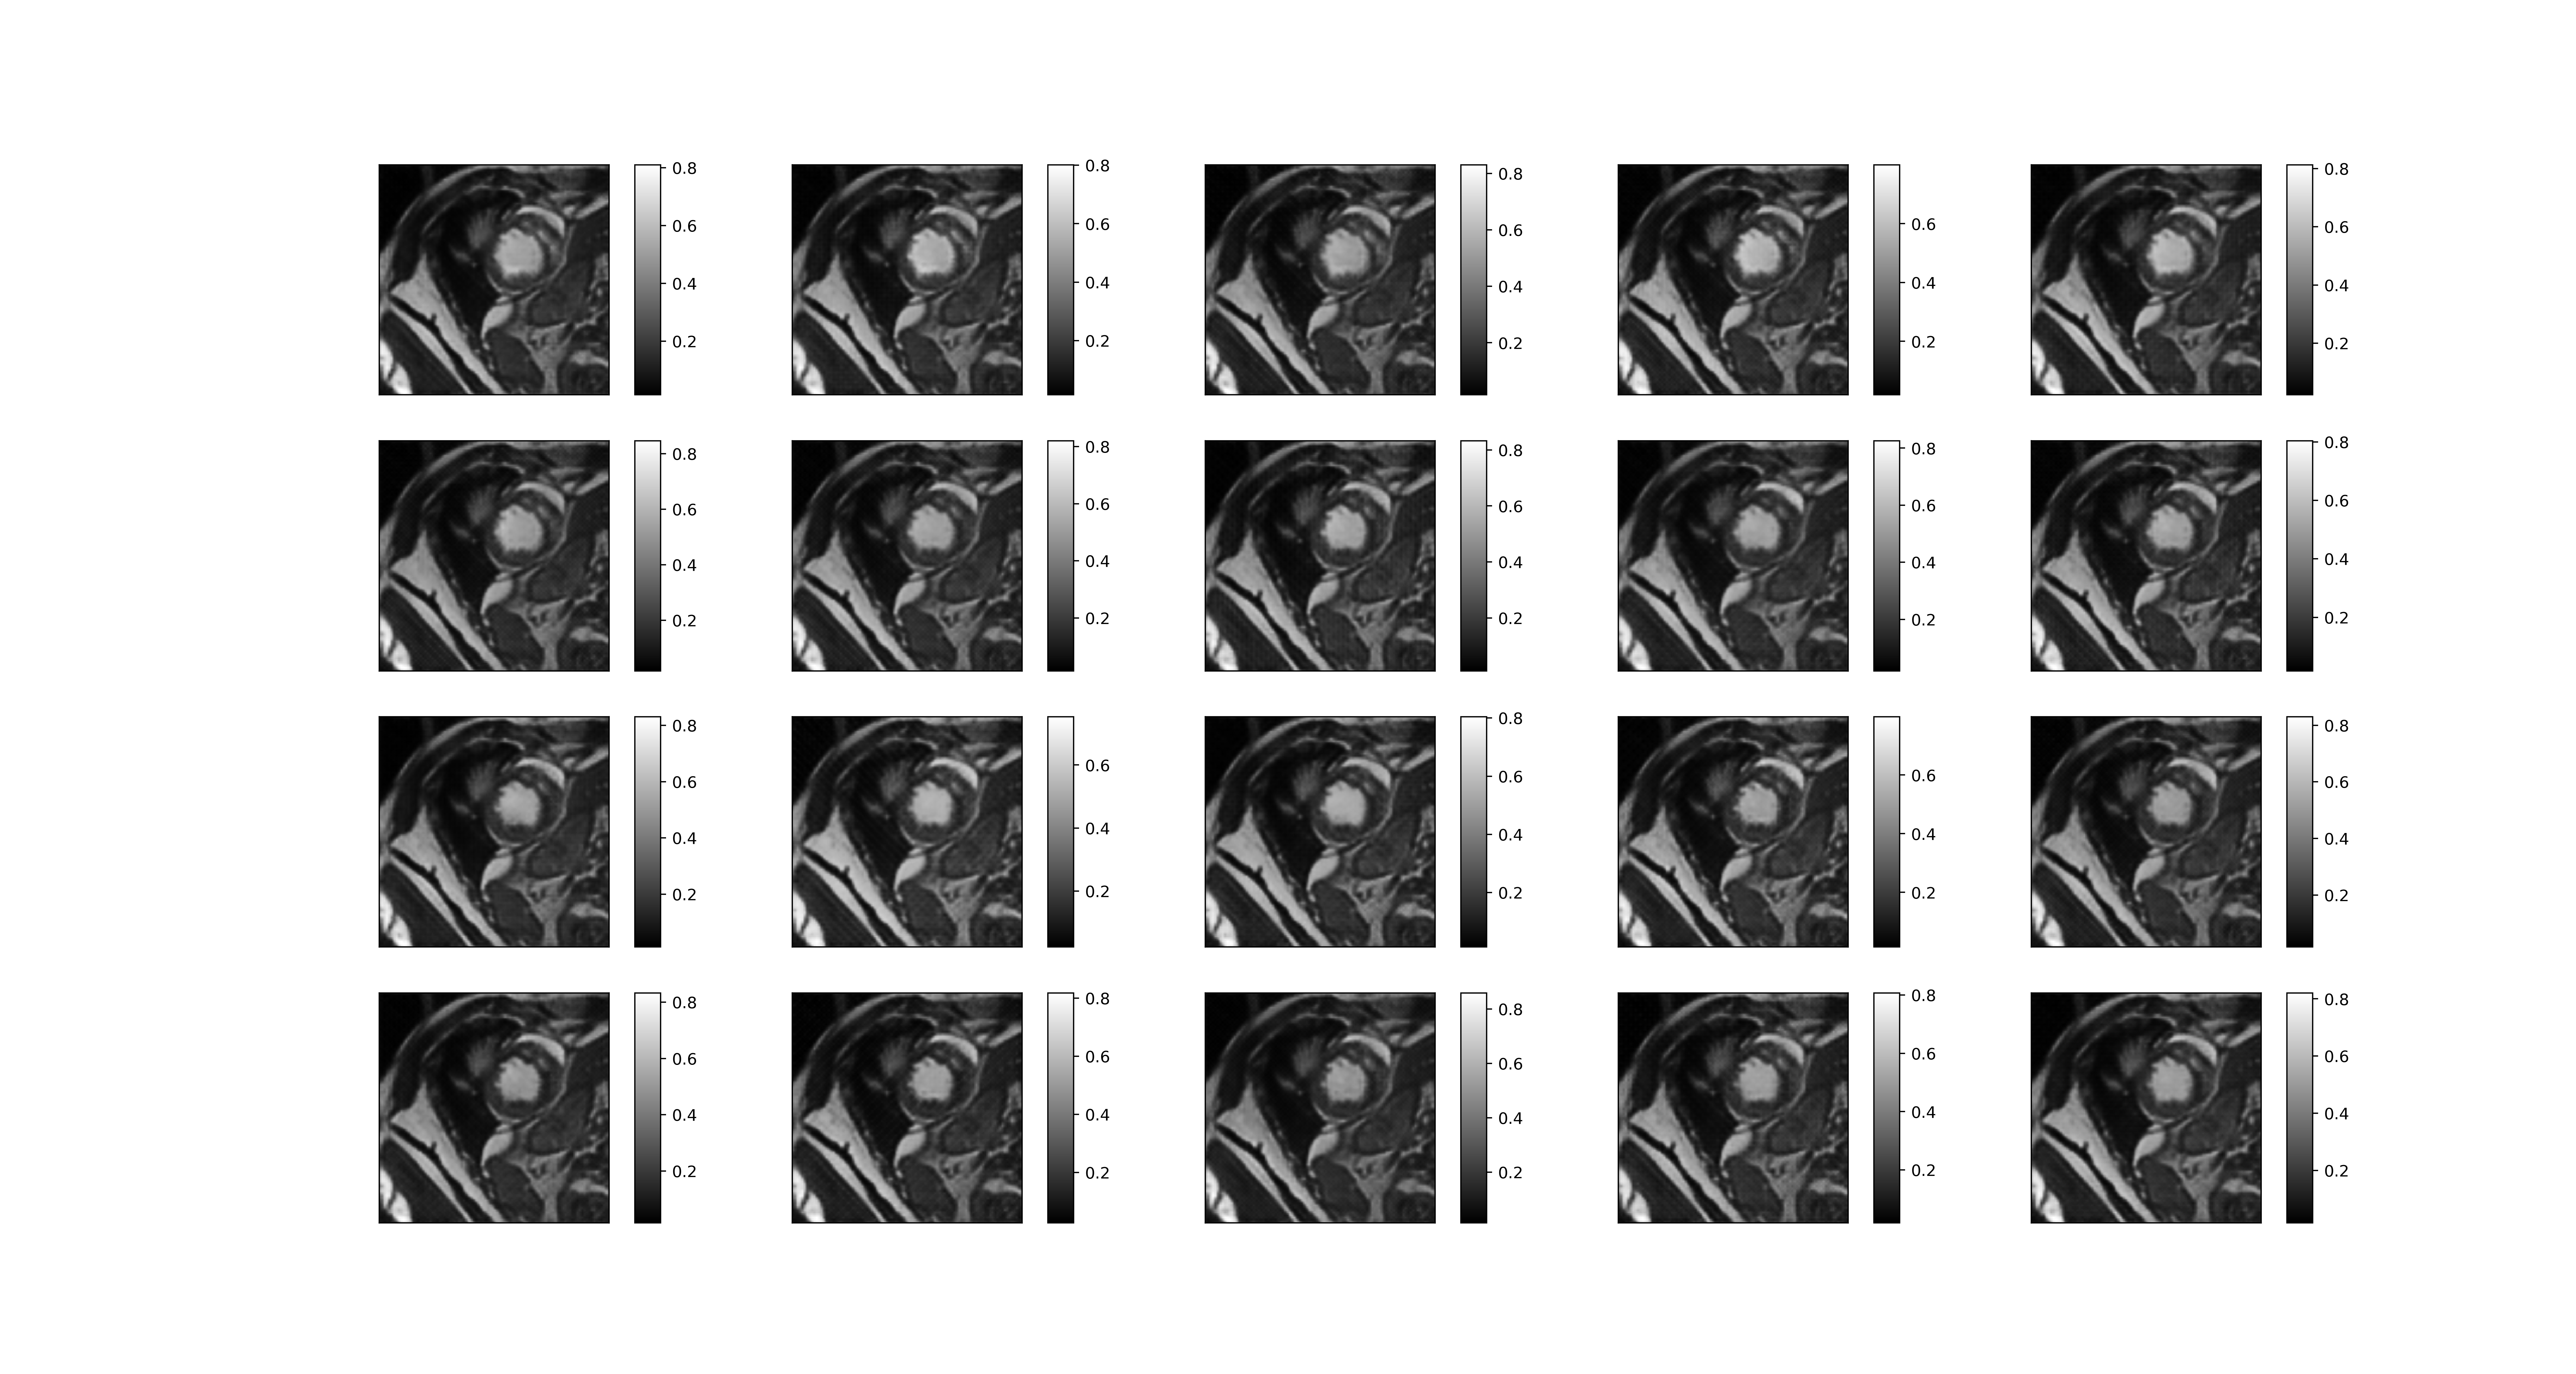
\includegraphics[width=\linewidth]{../images/output/reconstruction/reconstruction_2.png}
    \caption{reconstruction image 2}
  \end{subfigure}
  \caption{Reconstruction Images}
\end{figure}

Comment on the denoising/dealiasing performance:
\begin{enumerate} 
  \item Denoising: The network significantly reduces random noise in the input image,
        smoothing the image while protecting important structural features such as edges and details.
  \item Dealiasing: Our network reduces aliasing artefacts and enhances the realism of image
        textures and structures, avoiding unnatural distortions such as “streaks” and “swirls”.
\end{enumerate}

\subsection{Quantitative Evaluation}
We can calculate the PSNR and SSIM for each testing slice before and after deep
learning reconstruction. 
% TODO: write the path of the outcome and report the mean and 
% standard deviation of the PSNR and SSIM considering all the testing.



\section{Impact of Dropout and Dynamic Learning Rate}
We add drop out to our network training, and the code can be found in \texttt{class UNet}.
And a cosine annealing learning rate schedule with warm-up is employed, which can be
found in \texttt{function train()}.
% TODO: Compared to the baseline, this improves PSNR and SSIM by ....



\section{Compare L1 with L2}
We replace the L2 loss with L1 loss in the training pipeline,
retrain using the same architecture and training parameters.

% TODO: The L1-trained model ... in  PSNR and SSIM, suggesting ...



\section{Unrolled Deep Learning Reconstruction Network}
% TODO: 

\section{Tips for writing}
\label{tips}


\subsection{Headings: second level}
\subsubsection{Headings: third level}



\subsection{Footnotes}

\footnote{As in this example.}

\subsection{Figures}

% \begin{figure}
%   \centering
%   \fbox{\rule[-.5cm]{0cm}{4cm} \rule[-.5cm]{4cm}{0cm}}
%   \caption{Sample figure caption.}
% \end{figure}


\subsection{Tables}

% \begin{table}
%   \caption{Sample table title}
%   \label{sample-table}
%   \centering
%   \begin{tabular}{lll}
%     \toprule
%     \multicolumn{2}{c}{Part}                   \\
%     \cmidrule(r){1-2}
%     Name     & Description     & Size ($\mu$m) \\
%     \midrule
%     Dendrite & Input terminal  & $\sim$100     \\
%     Axon     & Output terminal & $\sim$10      \\
%     Soma     & Cell body       & up to $10^6$  \\
%     \bottomrule
%   \end{tabular}
% \end{table}


%%%%%%%%%%%%%%%%%%%%%%%%%%%%%%%%%%%%%%%%%%%%%%%%%%%%%%%%%%%%


\end{document}